%\documentclass[10pt, conference]{IEEEtran}
\documentclass[sigconf]{acmart}
%\pdfoutput=1
%\IEEEoverridecommandlockouts
% The preceding line is only needed to identify funding in the first footnote. If that is unneeded, please comment it out.
%\usepackage{cite}
\usepackage{amsmath,amssymb,amsfonts}
\usepackage{algorithmic}
\usepackage{graphicx}
\usepackage{textcomp}
\def\BibTeX{{\rm B\kern-.05em{\sc i\kern-.025em b}\kern-.08em
    T\kern-.1667em\lower.7ex\hbox{E}\kern-.125emX}}
\usepackage{multirow}
\usepackage{tabularx}
\usepackage{booktabs}
\usepackage{amsmath}
\usepackage{amsthm}
\usepackage{color}
\usepackage{enumitem}
\let\proof\relax
\let\endproof\relax
\usepackage{caption}
\usepackage{subcaption} 
%\captionsetup[table]{skip=10pt}
\usepackage{listings}
\usepackage{url}
\usepackage{pgfplots}
\usepackage{color}
\DeclareCaptionFormat{listing}{\colorbox{gray!50}{\parbox[l]{\columnwidth}{#1#2#3}}}
%\captionsetup[lstlisting]{format=listing,labelfont=black,textfont=black, font={footnotesize,black}}

\usepackage[]{algorithm2e}
\usepackage{algorithmic}
\renewcommand{\algorithmicrequire}{\textbf{Input:}}
\renewcommand{\algorithmicensure}{\textbf{Output:}}
\renewcommand{\algorithmicreturn}{\textbf{Algorithm:}}
%\renewcommand{\baselinestretch}{0.915}

%\graphicspath{{figures/}{./}}
\newcommand{\ajitha}[1]{\textbf{\color{blue}AR:{#1}}}
\newcommand{\foivos}[1]{\textbf{\color{blue}FT:{#1}}}
\newcommand{\miltos}[1]{\textbf{\color{blue}MA:{#1}}}
\newtheorem{ques}{Q}
\newtheorem{common}{C}

%TODOs
\newcommand{\todov}[1]{{\par\noindent\small\color{red} \framebox{\parbox{\dimexpr\linewidth-2\fboxsep-2\fboxrule}{\textbf{TODO:} #1}}}}

\lstset{language=C++,basicstyle=\footnotesize\ttfamily,breaklines=true}
\lstset{frame=tb,framextopmargin=50pt,frame=bottomline}

\begin{document}
 
\copyrightyear{2021}
\acmYear{2021}
\setcopyright{acmlicensed}\acmConference[SAC '21]{The 36th ACM/SIGAPP
	Symposium on Applied Computing}{March 22--26, 2021}{Virtual Event,
	Republic of Korea}
\acmBooktitle{The 36th ACM/SIGAPP Symposium on Applied Computing (SAC'21), March 22--26, 2021, Virtual Event, Republic of Korea}
\acmPrice{15.00}
\acmDOI{10.1145/3412841.3442027}
\acmISBN{978-1-4503-8104-8/21/03}

\title{Supervised Learning over Test Executions as a Test Oracle}\thanks{This work was supported by the Engineering and Physical Sciences Research Council (grant EP/L01503X/1), EPSRC Centre for Doctoral Training in Pervasive Parallelism at the University of Edinburgh, School of Informatics.}

\author{Foivos Tsimpourlas}
\email{F.Tsimpourlas@sms.ed.ac.uk}
\affiliation{
	\institution{University of Edinburgh}
	\country{}
}

\author{Ajitha Rajan}
\email{arajan@ed.ac.uk}
\affiliation{
	\institution{University of Edinburgh}
	\country{}
}

\author{Miltiadis Allamanis}
\email{miallama@microsoft.com}
\affiliation{
	\institution{Microsoft Research}
	\country{}
}


\iffalse
\author{\IEEEauthorblockN{Foivos Tsimpourlas}
	\IEEEauthorblockA{\textit{University of Edinburgh} \\
		F.Tsimpourlas@sms.ed.ac.uk}
	\and
	\IEEEauthorblockN{Ajitha Rajan}
	\IEEEauthorblockA{\textit{University of Edinburgh} \\
		arajan@ed.ac.uk}
	\and
	\IEEEauthorblockN{Miltiadis Allamanis}
	\IEEEauthorblockA{\textit{Microsoft Research} \\
		miallama@microsoft.com}
}
\fi

%\maketitle


%%%%
%Include here the files for each chapter
%%%%
\begin{abstract}


%A key activitiy in software testing is determining the correctness of test executions, that is currently an expensive and error prone
%manual activity.   
The challenge of automatically determining the correctness of test executions is referred to as the \emph{test oracle problem} and is a
key remaining issue for automated testing.
The paper aims at solving the test oracle problem in a scalable and accurate way. 
To achieve this, we use supervised learning over test execution traces. We label a small fraction of the execution traces with their verdict of pass or fail. 
We use the labelled traces to train a neural network (NN) model to learn to distinguish runtime patterns for passing versus failing executions for a given program. 

We evaluate our approach using case studies from different application domains - 1. Module from Ethereum Blockchain, 2. Module from PyTorch deep learning framework, 3. Microsoft SEAL encryption library components and 4. Sed stream editor. We found the classification models for all subject programs resulted in high precision, recall and specificity, averaging to 89\%, 88\% and 92\% respectively, while only training with an average 15\% of the total traces. Our experiments show that the proposed NN model is promising as a test oracle and is able to learn runtime patterns to distinguish test executions for systems and tests from different application domains. 

%\begin{IEEEkeywords}
%component, formatting, style, styling, insert
%\end{IEEEkeywords}

%This is the abstract
\end{abstract}

\maketitle

\section{Introduction}
\label{sec:intro}

As the scale and complexity of software increases, the number of tests needed for effective validation becomes extremely large, 
slowing down development, hindering programmer productivity, and ultimately making development costly~\cite{ammann2016introduction}.
To make testing faster, cheaper and more reliable, it is desirable to automate as much of the process as possible. 
%The need for large numbers of tests is magnified in agile software development practices, 
%like Continuous Integration (CI) and Test-Driven Development (TDD), that require extensive testing to be performed~\cite{humble2010continuous}.
%Google using CI development for its products reports a need for running large numbers of tests every day (more than $100$ million tests per day)~\cite{kumar2010development}. 

Over the past decades, researchers have
made remarkable progress in automatically generating effective test inputs~\cite{chen2013orchestrated, bertolino2007software}. Automated test input generation tools, however, generate substantially more tests than manual approaches. This becomes an issue when determing the correctness of test executions, a procedure referred to as the \emph{test oracle}, that is still largely manual, relying on developer expertise.  Recent surveys on the test oracle problem~\cite{barr2015oracle, nardi2015survey, langdon2017inferring} show that automated oracles based on formal specifications, metamorphic relations~\cite{liu6613484} and independent program versions are not 
widely applicable and difficult to use in practice. 
In this paper, we seek to address the test oracle problem. More specifically, for a system with a large set of test inputs, that are automatically 
%~\cite{Chung2009GeneratingID, Chung2004ASA, Huang6340123, lipka7302457} 
and/or manually generated, we ask,  \\ 
\emph{`` Is there a widely applicable technique that automates the classification of test executions as pass/fail ? ''}
%One of the biggest hurdles in test automation is the \emph{test oracle} - ``a procedure that distinguishes between the correct and incorrect behaviours of the System Under Test (SUT)''~\cite{barr2015oracle}.  Literature refers to the challenge of automatically determining the correctness of test executions as the \emph{test oracle problem} and acknowledges it as one of the key  
%remaining issues for automated testing~\cite{barr2015oracle}. 
%Recent surveys on the test oracle problem~\cite{barr2015oracle, nardi2015survey, langdon2017inferring} 
%show that existing techniques based on formal specifications, metamorphic relations and independent program versions are not 
%widely applicable and difficult to use in practice. 
%todov{Elaborate on limitations of existing oracles.}
\begin{figure*}[h]
	\centering
	\includegraphics[scale=0.35]{../../figures/key_idea.png}
	\vspace{-6pt}
	\caption{Key idea in our approach.}
%	\vspace{-20pt}
	\label{fig:key-idea}
	\vspace{-8pt}
	%\Description[\texttt{Encoder 2} representing a sequence of trace lines and global state as a single vector.]
\end{figure*}

\textbf{Key Idea.}
We explore supervised machine learning to infer a test oracle from labelled execution traces of a given system. %, using neural networks (NNs).
%In particular, we use neural networks (NNs), well suited to learning complex functions, to design the test oracles. %tailored to each software, using neural networks that have been.  
In particular, we use neural networks (NNs), well suited to learning complex functions and classifying patterns, to design the test oracles.
Our technique is widely applicable and easy to use, as it only requires execution traces gathered from running tests through the program under test (PUT) to design the oracle. This is shown in Figure~\ref{fig:key-idea} where a small fraction of the gathered execution traces labelled with pass/fail (shown in light gray) is used to train the NN model which is then used to automatically classify the remaining unseen execution traces (colored dark gray). 

Previous work exploring the use of NNs for test oracles has been in a restricted context -- applied to very small programs with primitive data types, and only considering their inputs and outputs~\cite{vanmali2002using, jin2008artificial}. Information in execution traces which we believe is useful for test oracles has not been considered by existing NN-based approaches.
Other bodies of work in program analysis have used NNs
%Recent work using NNs over programs 
to predict method or variable names and detecting name-based bug patterns~\cite{alon2018code2vec, pradel2018deepbugs} relying on static program information, namely,  embeddings of the Abstract Syntax Tree (AST) or source code. %Automated generation of labelled data has also been overlooked. 
Our proposed approach is the first attempt at using \emph{dynamic execution trace information in NN models for classifying test executions}.

Our approach for inferring a test oracle has the following steps, 
\begin{enumerate}[itemsep = 0pt, topsep = 0pt, partopsep=0pt]
\item Instrument a program to gather execution traces as sequences of method invocations. %record method calls, arguments, and return values for every test execution, 
\item Label a small fraction of the traces with their classification decision. %The labelled traces are used to train the NN model.
\item Design a NN component that embeds the execution traces to fixed length vectors.
\item Design a NN component that uses the line-by-line trace information to classify traces as pass or fail.
\item Train a NN model that combines the above components and evaluate it on unseen execution traces for that program. 
\end{enumerate}
The novel contributions in this paper are in Steps 3, 4 and 5. Execution traces from a program vary widely in their length and information. We propose a technique to encode and summarise the information in a trace to a fixed length vector that can be handled by a NN. We then design and train a NN to serve as a test oracle.  
%The novelty in our approach lies in using execution traces to train and build a NN model for test classification.  


\textbf{Labelled execution traces.} Given a PUT and a test suite, we gather execution traces corresponding to each of the test inputs in the test suite with our instrumentation framework. Effectively learning a NN classifier for a PUT that distinguishes correct from incorrect executions requires labelled data with both passing and failing examples of traces. 
We require a small fraction of the overall execution traces to be labelled, which is likely to be a manual process. 
As a result, our proposed approach for test oracle is \emph{not} fully automated.
%For example, 10\% of the test execution traces, the remaining 90\% of execution traces will be automatically classified by our approach. %In our experiments, we report the effect of training data size on verdict (passing or failing) prediction accuracy. 
We hypothesize that the time invested in labelling a small proportion of the traces is justified with respect to the benefit gained in automatically classifying the remaining majority of traces. 
In contrast, with no classifier, the developer would have had to specify expected output for all the tests, which is clearly more time consuming than the small proportion of tests we need labelled. 

%Our technique is not fully automated as it relies on training with labelled traces, where labelling is likely to be a manual process. T
%It is common for case studies to have many passing test inputs but only a limited number of failing tests. To address this imbalance in training, we mutate the reference code with common bugs. Test inputs are labelled as passing traces if their output matches the expected output. Otherwise, they are labelled as failing traces.


% To address this imbalance in training, we generate failing traces by mutating the existing code with common bugs. Test inputs that were labelled with passing traces through the original code will be labelled with failing traces through the mutated code if the output deviates from the expected output. %from passing test inputs by mutating the source code. 


\textbf{NN Architecture.} 
An execution trace in our approach comprises multiple lines, with each line containing information on a method invocation. 
Our architecture for encoding and classifying an execution trace uses multiple components: (1) Value encoder for encoding values within the trace line to a distributed vector representation, (2) Trace encoder encoding trace lines within a variable-length trace to a single vector, and (3) Trace Classifier that accepts the trace representation and classifies the trace. The components in our architecture is made up of LSTMs, one-hot encoders, and a multi-layer perceptron. 

\textbf{Case Studies.} We evaluate our approach using 4 subject programs and tests from different application domains - a single module from Ethereum project~\cite{ethereum}, a module from Pytorch~\cite{pytorch}, one component within Microsoft SEAL encryption library~\cite{sealcrypto} and a Linux stream editor~\cite{sed}.  
One of the 4 subject programs were accompanied by both passing and failing tests that we could directly use in our experiment. The remaining three programs were only accompanied by passing tests. We treated these programs as reference programs. We then generated PUTs by artificially seeding faults into them. We generated traces through the PUTs using the existing tests, labelling the traces as passing or failing based on comparisons with traces from the reference program.  We trained a NN model for each PUT using a fraction of the labelled traces. We found our approach for designing a NN classification model was effective for programs from different domains. We achieved high accuracies in detecting both failing and passing traces, with an average precision of 89\% and recall of 88\%. Only a small fraction of the overall traces (average 15\%) needed to be labelled for training the classification models.
%For most subject programs, this fraction was 10\% of the total traces.  

\noindent In summary, the paper makes the following contributions:
\begin{itemize}[itemsep = 0pt, topsep = 0pt, partopsep=0pt]
\item Given a PUT and its test inputs, we provide a framework that instruments the PUT and gathers test execution traces as sequences of method invocations. 
\item A NN component for encoding variable-sized execution traces into fixed length vectors.
\item A NN for classifying the execution traces as pass or fail.  
\item We provide empirical evidence that this approach yields effective test oracles for programs and tests from different application domains. 
\end{itemize}
\vspace{-5pt}





%\vspace{10pt} 
 \section{Background}
 \label{sec:background}
When a test oracle observes a test execution, it returns a
test verdict, which is either pass or fail, depending on whether the observations match 
expected behaviour. A test execution is execution of the PUT with a test input. The importance of oracles as an integral part of the testing process has been a key topic of research for over three decades. 
We distinguish four different kinds of test oracles,
based on the survey by Barr et al.~in 2015~\cite{barr2015oracle}. The most common form of test oracle is a \emph{specified oracle},
one that judges behavioural aspects of the system under test
with respect to formal specifications. Although formal specifications are effective in identifying failures,  
defining and maintaining such specifications is expensive
and also relatively rare in practice.
\emph{Implicit} test oracles require no domain knowledge and 
are easy to obtain at no cost. However, they are
limited in their scope as they are only able to reveal  particular anomalies like buffer overflows, segmentation faults, deadlocks. 
\emph{Derived} test oracles use 
documentations or system executions, to judge a system's behaviour,
when specified test oracles are unavailable. 
However, derived test oracles, like metamorphic relations and inferring invariants, is either not automated  
or it is inaccurate and irrelevant making it challenging to use.

For many systems and much of
testing as currently practised in industry, the
tester does not have the luxury of formal specifications or assertions or even automated partial
oracles~\cite{hierons2009verdict, hierons2012oracles}. %The tester must therefore
%face the potentially daunting task of manually
%checking the system’s behaviour for all test
%cases generated. 
Statistical analysis and machine learning techniques provide a useful alternative for understanding software behaviour using data 
gathered from a large set of test executions.
%We plan to use neural networks (NNs), well suited to learning complex functions, to design the test oracles. %tailored to each software, using neural networks that have been.  
%We believe NNs would be a good fit as it can help learn to identify high-level features of the program state 
%that indicate correct versus incorrect test executions. 
%There has been some work exploring the use of NNs, in a restricted context, for correctness checks. 

\subsection{Machine Learning for Software Testing}
Briand et al.~\cite{briand2008novel}, in $2008$, presented a comprehensive overview of existing techniques that apply machine learning for addressing testing challenges.
Among these, the closest related work is that of
Bowring et al.\ in $2004$~\cite{bowring2004active}. They proposed an active learning approach to
build a classifier of program behaviours using a frequency profile of single events in the
execution trace. %They learn two sets of first-order Markov models,
%where each set characterizes correct and incorrect behaviors separately. 
%Their approach is only applicable if event transition profiles produced by a program can be encoded as a Markov model. 
Evaluation of their approach was conducted over one small program whose specific structure was well suited to their technique. 
%Their technique for building markov models wiill not scale to programs with large number of states. 
%applying this technique over programs with large numbers of states is not clear and the authors only  evaluated their techover a single small program.
Machine learning techniques have also been used in fault detection. 
Brun and Ernst, in $2004$~\cite{brun04finding}, explored the use of support vector machines and decision trees to rank program properties, provided by the user,  that are likely to indicate 
errors in the program. Podgurski et al., in $2003$~\cite{podgurski2003automated},
%use cluster analysis techniques on passing and failing execution profiles to help debugging. 
use clustering
over function call profiles to determine which failure reports
are likely to be manifestations of an underlying error. A training step determines which features are of interest
by evaluating those that enable a model to distinguish
failures from non-failures. The technique does not
consider passing runs. In their experiments, most
clusters contain failures resulting from
a single error.
%Engler et al., in $2001$~\cite{engler01bugs}, used statistical ranking to 
%automatically extract programmer beliefs from source code and flag belief contradictions as errors. 
%The goal of their work is different from ours in that they focus on error detection. They propose techniques to infer properties of programs that are likely to lead to errors 
%so that the programmer only needs to examine those propoerties to locate an error. 

More recently, Almaghairbe et al.~\cite{almaghairbe2017separating} proposed an unsupervised learning technique to classify unlabelled execution traces of simple programs. They gather two kinds of execution traces, one with only inputs and outputs, and another that includes the sequence of method entry and exit points, with only method names. Arguments and return values are not used. %over three different subject programs. They evaluated their technique on two types of traces, the first including traces that contain only the input and output of a program, while the second included state invariants as well. Then, clustering was used to organize the traces into clusters, using a set of different algorithms. 
They use agglomerative hierarchical clustering algorithms to build an automated test oracle, assuming passing traces are grouped into large, dense clusters and failing traces into many small clusters. They evaluate their technique on 3 programs from the SIR repository~\cite{sir}. The proposed approach has several limitations. They only support programs with strings as inputs. 
They do not consider correct classification of passing traces.
The accuracy achieved by the technique is not high, classifying approximately 60\% of the failures. Additionally, fraction of outputs that need to be examined by the developer is around 40\% of the total tests, which is considerably higher than the labelled data used in our approach. 
%In Section~\ref{sec:resuls}, we present 
We objectively compared the accuracy achieved by the hierarchical clustering technique against our approach using 5 PUTs, discussed in Section~\ref{sec:results}. We found our approach achieves significantly higher accuracy in classifying program executions across all case studies. 
%Number of clusters and threshold cluster size for failure clusters needs to be empirically determined for each program. 

\iffalse
Almaghairbe et al. assumed that all the passing traces present the same behaviour, leading to them being organized in one, large cluster. On the other hand, according to them, failing traces tend to present non-uniform, wide-ranging patterns, which results in failing traces being spread among many small clusters. According to their methodology, the clusters that are sized below the average of the set, are considered to contain failing traces and clusters sized above the average are considered to contain passing traces. For their evaluation, they used different clustering techniques and experimented on multiple cluster sizes. Almaghairbe et al. used `Daikon' for instrumentation, an invariant detector that uses machine learning to observe program values and summarize them into a set of formulas.

\foivos{I am writing their weaknesses in items and then we will place them into the text.}

\textcolor{blue}{Almaghairbe et al. weaknesses:
\begin{enumerate}
	\item They assume that small failing traces present diverging features, which is not always true. They also assume that passing traces have the same pattern, which is also most of the times wrong.
	\item Their technique is based on programs that actually give an output. Not only that, but as they state at the end of the paper, ``the input/output pairs of the subject programs were string data". Their methodology is not applicable to programs with different data types other than strings, or to programs that only differ in their internal states and do not give a visible output to the user.
	\item They only evaluate on 3 use cases and their precision numbers in almost every case is nowhere near good to be used on a real scenario. To get good precision numbers they combine clustering techniques, linkage types, clustering sizes, multiple versions for the same program. So many combinations and still it seems to underperform.
	\item Their instrumentation is language specific. They used C and Java. Daikon (the instrumentation tool) only supports C, Java, Lisp, Javascript. LLVM is language agnostic.
	\item Daikon by itself is inaccurate (as they state at the faq of its page, it suffers from false negatives due to having a simple grammar).
	\item Their clustering works by grouping a limited number of categorical outputs (different strings). What if their outputs were numerical ?
	\item There are 2-3 cases in which they present 100\% precision and 1 F1 score. This happened because apparently one of the many clustering combinations they used for the program, grouped only the passing traces into one large cluster and only the failing traces into many small clusters. But this was just an exception to the normal case. Their technique is not applicable to a real life scenario: if they were to classify NanoXML without knowing the label of the traces (this is what the paper claims) which technique would they use, when only one works out of so many ?
\end{enumerate}}

\foivos{End}
\fi

%, Bug detection work by Pradel and Sen} 
%Fault detection in these techniques is applied once the tester knows an execution has failed. The goal in our work is to provide the tester with this knowledge of failing executions. 
%Detecting faults in programs that cause test failures is different, but complementary to our goal of classifying test executions. 
Existing work using execution traces for bug detection has primarily been based on clustering techniques. Neural networks, especially with deep learning, have been very successful for complex classification problems in other domains like natural language processing, speech recognition, computer vision. There is limited work exploring their benefits for software testing problems.  


\paragraph{Neural Networks for Test Oracles} 
NNs were first used by Vanmali et al.~\cite{vanmali2002using} in 2002 to simulate behaviour of simple programs
using their previous version, and applied this model to regression testing of unchanged functionalities. 
Aggarwal et al.~\cite{aggarwal2004neural} and Jin et al.~\cite{jin2008artificial} applied the same approach to test a triangle classification program, that computes the relationship among three edge inputs to determine the type of triangle. 
The few existing approaches using NNs have been applied to simple programs having small I/O domains.
The following challenges have not been addressed in existing work, \\ 
%\begin{enumerate}
 \noindent 1. Training with test execution data and their vector representation -- Existing work only considers program inputs and outputs that are of primitive data types (integers, doubles, characters). %Complex input/output data types and program paths and states taken during execution have not been previously explored. 
 Test data for real programs often use complex data structures and data types defined in libraries. There is a need for techniques that encode such data. In addition, existing work has not attempted to use program execution information in NNs to classify tests.  Achieving this will require novel techniques for encoding execution traces and designing a NN that can learn from them.    \\
 %Techniques for encoding intermediate states during program execution has not been considered previously. 
 \noindent 2. Test oracles for industrial case studies - Realistic programs with complex behaviours and input data structures has not been previously explored. \\
 \noindent 3. Effort for generating labelled training data - Training data in existing work has been over simple programs, like the triangle classification program, where labelling the tests was straightforward. Availability of labelled data that includes failing tests has not been previously discussed. Additionally, the proportion of labelled data needed for training and its effect on model prediction accuracy has not been systematically explored. 

 \paragraph{Deep Learning for Software Testing}
 The performance of neural networks as classifiers was boosted with the birth of deep learning in 2006~\cite{hinton2006fast}.
 Deep learning methods have \emph{not} been explored extensively for software testing, and in particular for the test oracle problem.
 Recently, a few techniques have been proposed for automatic pattern-based bug detection. For example, 
 Pradel et al.~\cite{pradel2018deepbugs} proposed a deep learning-based static analysis for automatic name-based bug detection and
 Allamanis et al.~\cite{allamanis2018learning} used graph-based neural static analysis for detecting variable misuse bugs. 
In addition to these techniques, several other deep learning methods for statically representing code have been developed~\cite{alon2018code2seq,allamanis16convattn}. 
We do not discuss these further since we are interested in execution trace classification and in NNs that use dynamic trace information rather than a static view of the code.

 \iffalse
 %%%%Deep Learning to find bugs%%%%%%%%%%55
They present an approach for automatic bug detection using neural networks that are trained to distinguish buggy from non-buggy code. 
 To generate large numbers of positive and negative training samples, 
code transformations are used to create incorrect code from existing code samples. 
Input to the NN is a translation of code as a vector. Vector representation of code
is based on the AST and uses a distributed embedding for identifiers where its context is the surrounding nodes in the AST - parent, grand parent, siblings, uncles, cousins. 
Each value in the context is a string value that represents the identifier name or literal name of that node. Vector representation of node is its one hot encoding. 
For the context, it's vector representation is a concatenation of its component vectors that are one hot encodings if it is a string and single element if it is position.  
Based on the vector representation of code, 
a bug detector is a model that distinguishes
between vectors that correspond to correct and incorrect code examples.
The authors create four bug detectors for JavaScript - accidentally swapped function arguments, incorrect assignments, and incorrect binary operations.
\fi
 
 %
 % Different NN architectures, their parameters,  and how to select them based on the program and test data 
% characteristics is not well understood and remains unexplored. \\
% \noindent 1. Labelling test data - the training samples in existing work has been provided by domain experts with knowledge of expected output 
% or the program was simple enough like the triangle classification program that labelling the tests was straightforward. 
% The challenge in obtaining labelled training samples without relying on a human oracle for complex applications has not been addressed.  \\
%\noindent 2. Generating large numbers of training samples - Automated generation of large numbers of labelled test data and their representation for training %the NN has not been explored systematically. \\
 
%\end{enumerate}

\paragraph{Embedding Execution Traces for Neural Networks}
%\ajitha{Discuss the following} -  Simple NN model over execution traces, \\
%Recent learning-based approaches proposed for bug detection~\cite{} rely on using vector representations of program ASTs. There is limited work in using representations of execution traces.   
One of the main contributions in this paper is an approach for embedding information in execution traces as a fixed length vector to be fed into the neural network. There is limited work in using representations of execution traces. Wang et al.~\cite{wang2017dynamic} proposed embeddings of execution traces in 2017. They use execution traces captured as a sequence of variable values at different program points. A program point is when a variable gets updated. Their approach uses recurrent NNs to summarise the information in the execution trace. Embedding of the traces is applied to an existing program repair tool. The work presented by Wang et al. has several limitations - 1. Capturing execution traces as sequences of updates to every variable in the program has an extremely high overhead and will not scale to large programs. The paper does not describe how the execution traces are captured, they simply assume they have them. 2. The approach does not discuss how variables of complex data types such as structs, arrays, pointers, objects are encoded. It is not clear if the traces only capture updates to user-defined variables, or if system variables are also taken into account. 
%Information from system variables can be important in detecting bugs but is also accompanied by a high overhead in tracking them. 
3. The evaluation uses three simple, small  programs (eg. counting parentheses in a string) from students in an introductory programming course. %, generating digits in an integer, printing the chessboard pattern using ``X'' and ``O'' to represent the squares. 
The complexity and scale of real programs is not assessed in their experiments. Their technique for capturing and directly embedding traces as sequences of updates to every variable is infeasible in real programs. 
Our approach captures and embeds traces as sequences of method invocations and updates to global variables, which scales better than tracking every program variable. We have implemented our instrumentation in the LLVM compiler framework that is language agnostic and scales to industry-sized programs. We support all types of variables and objects, including system defined variables. %Our embedding technique for traces is completely different from Wang et al.~\cite{wang2017dynamic} as it encodes sequences of method invocations and global state. Our experiments show feasibility of our technique over large, real programs. 
%  https://rishabhmit.bitbucket.io/papers/dyn_iclr18.pdf
%  Neural network representations of LLVM use-def graphs}
%  https://papers.nips.cc/paper/7617-neural-code-comprehension-a-learnable-representation-of-code-semantics.pdf


%\section{Motivational Example}
%\label{sec:example}
%\input{Example}

\section{Approach}
 \label{sec:approach}
\begin{figure*}[t]
    \centering
    \begin{subfigure}[b]{0.5\textwidth}
        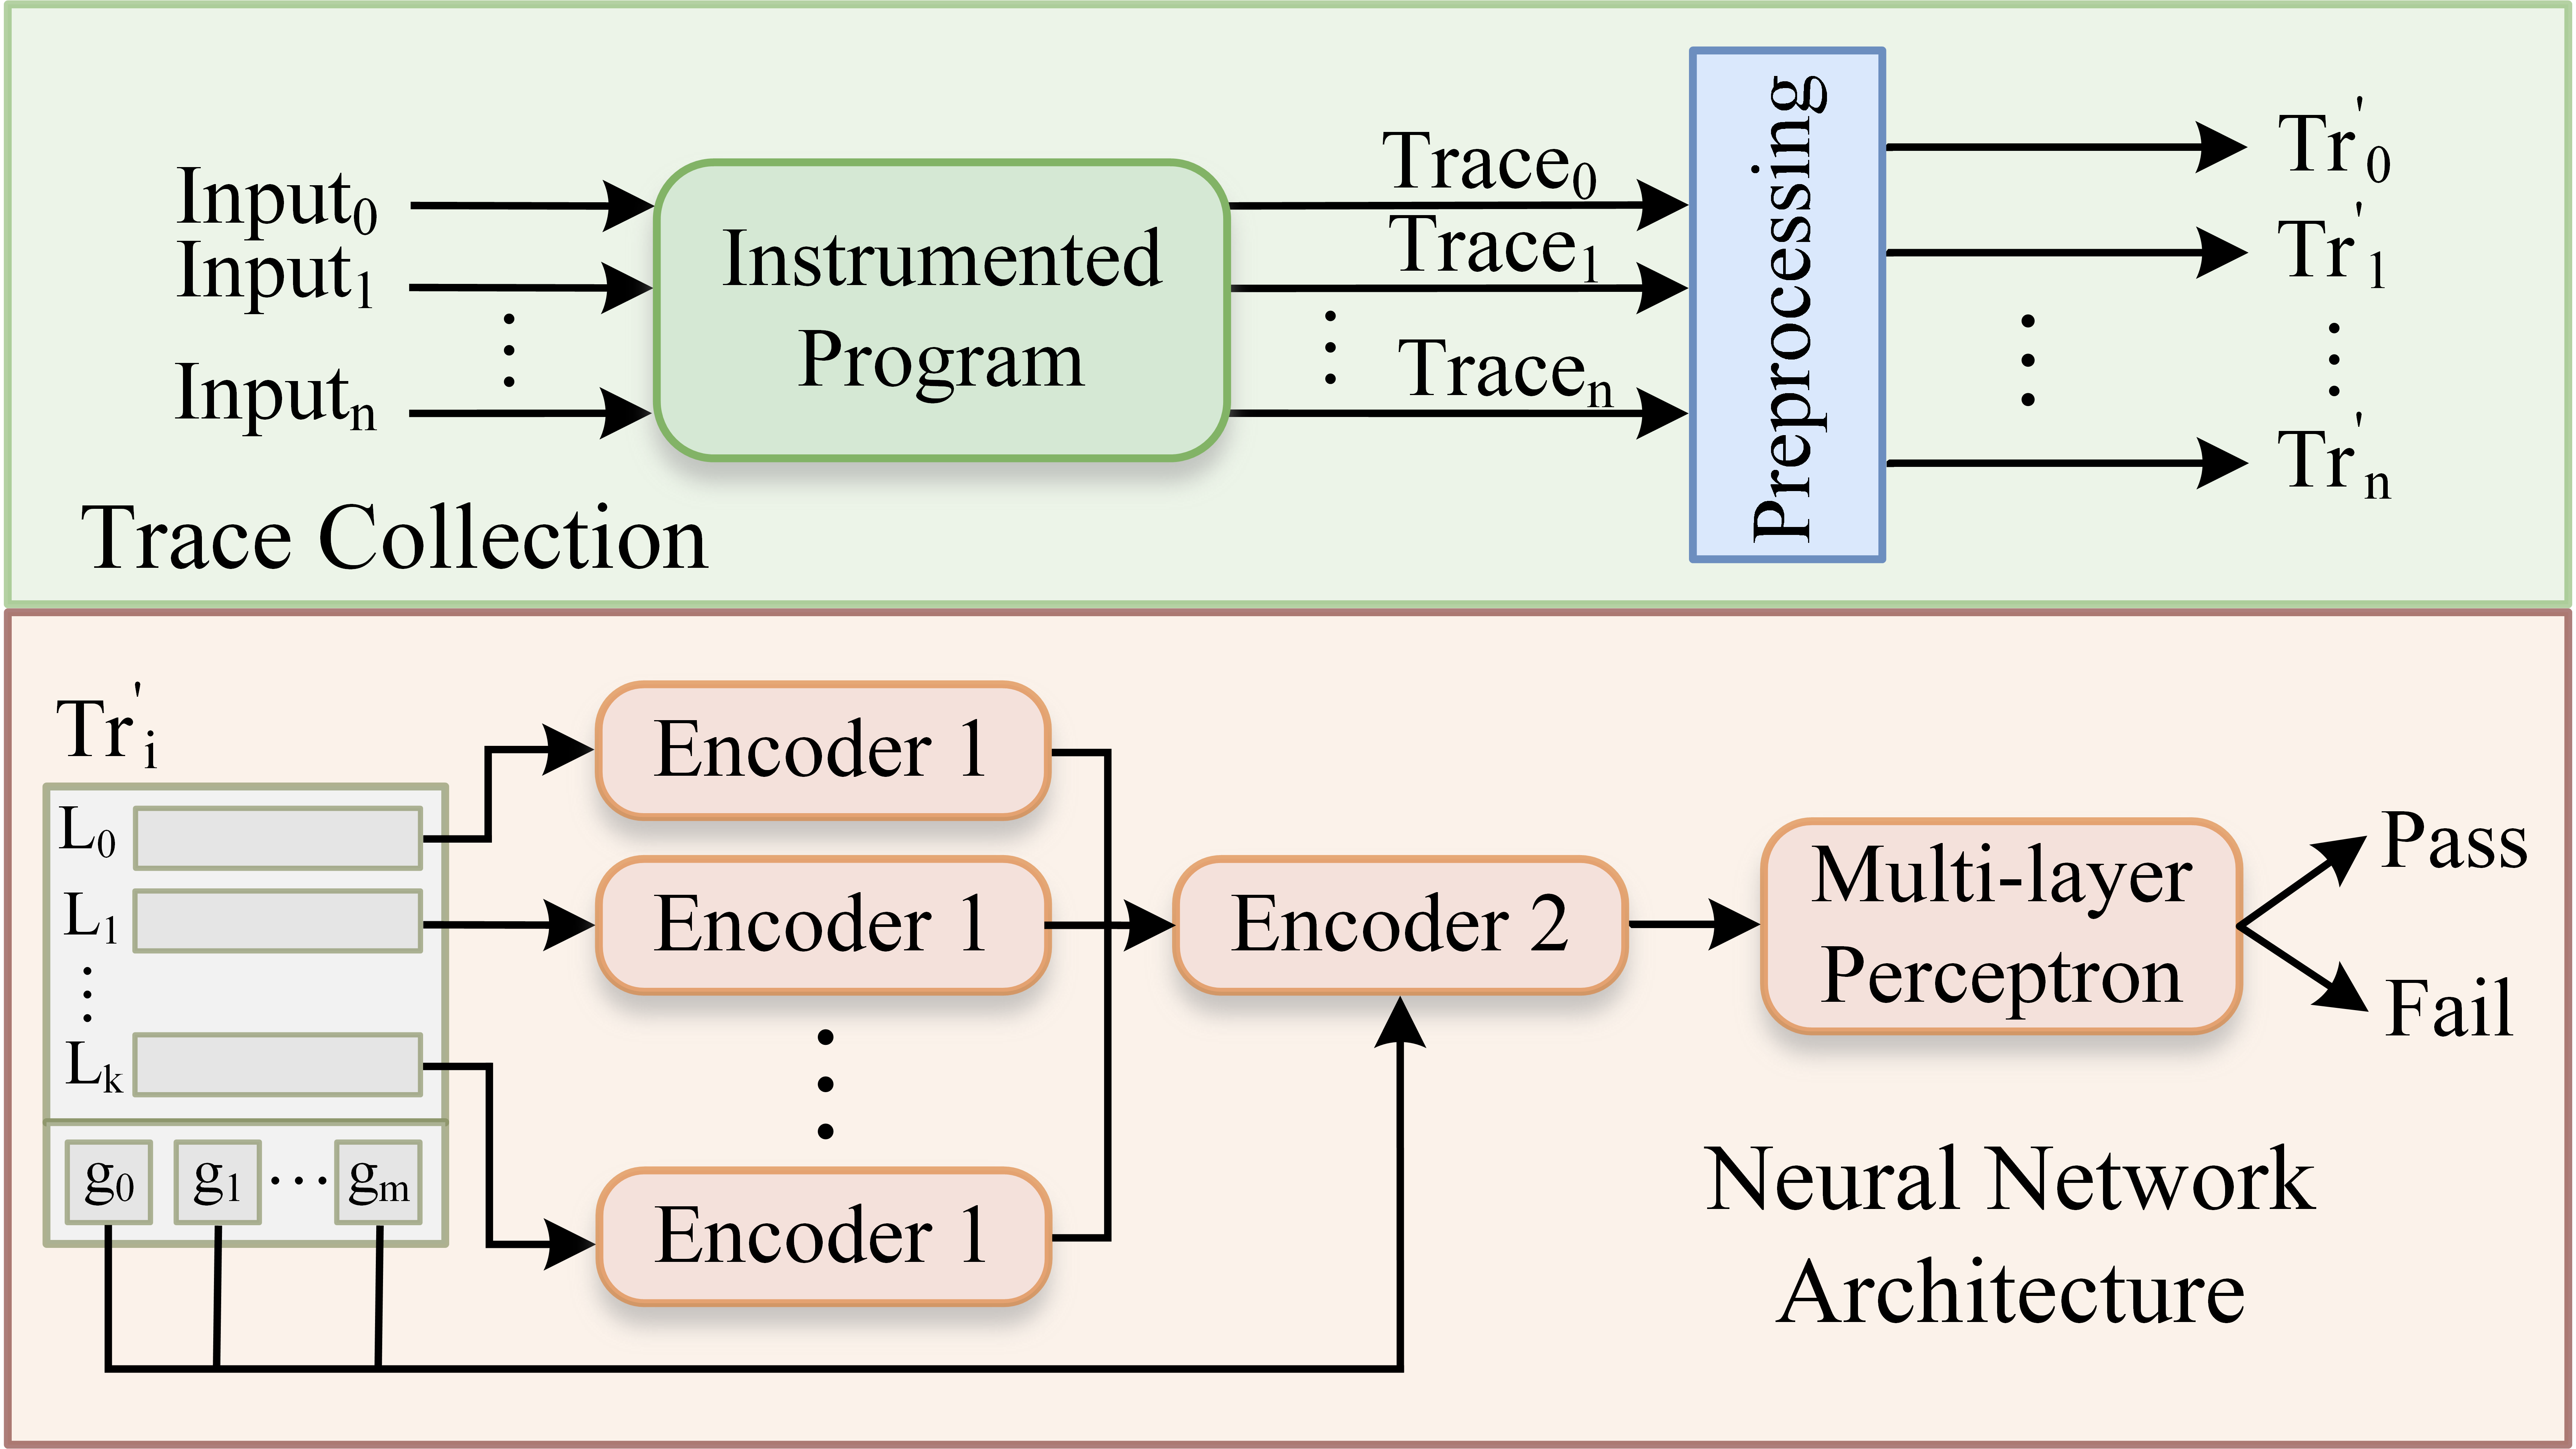
\includegraphics[scale=0.88]{../../figures/pipeline.png} %1.071
    %\vspace{-6pt}
    \caption{Gathering traces, encoding them, and using NNs to classify them.}
        %\vspace{0.5cm}
        \label{fig:pipeline}
    \end{subfigure}~~
    \centering
    \begin{subfigure}[b]{0.5\textwidth}
        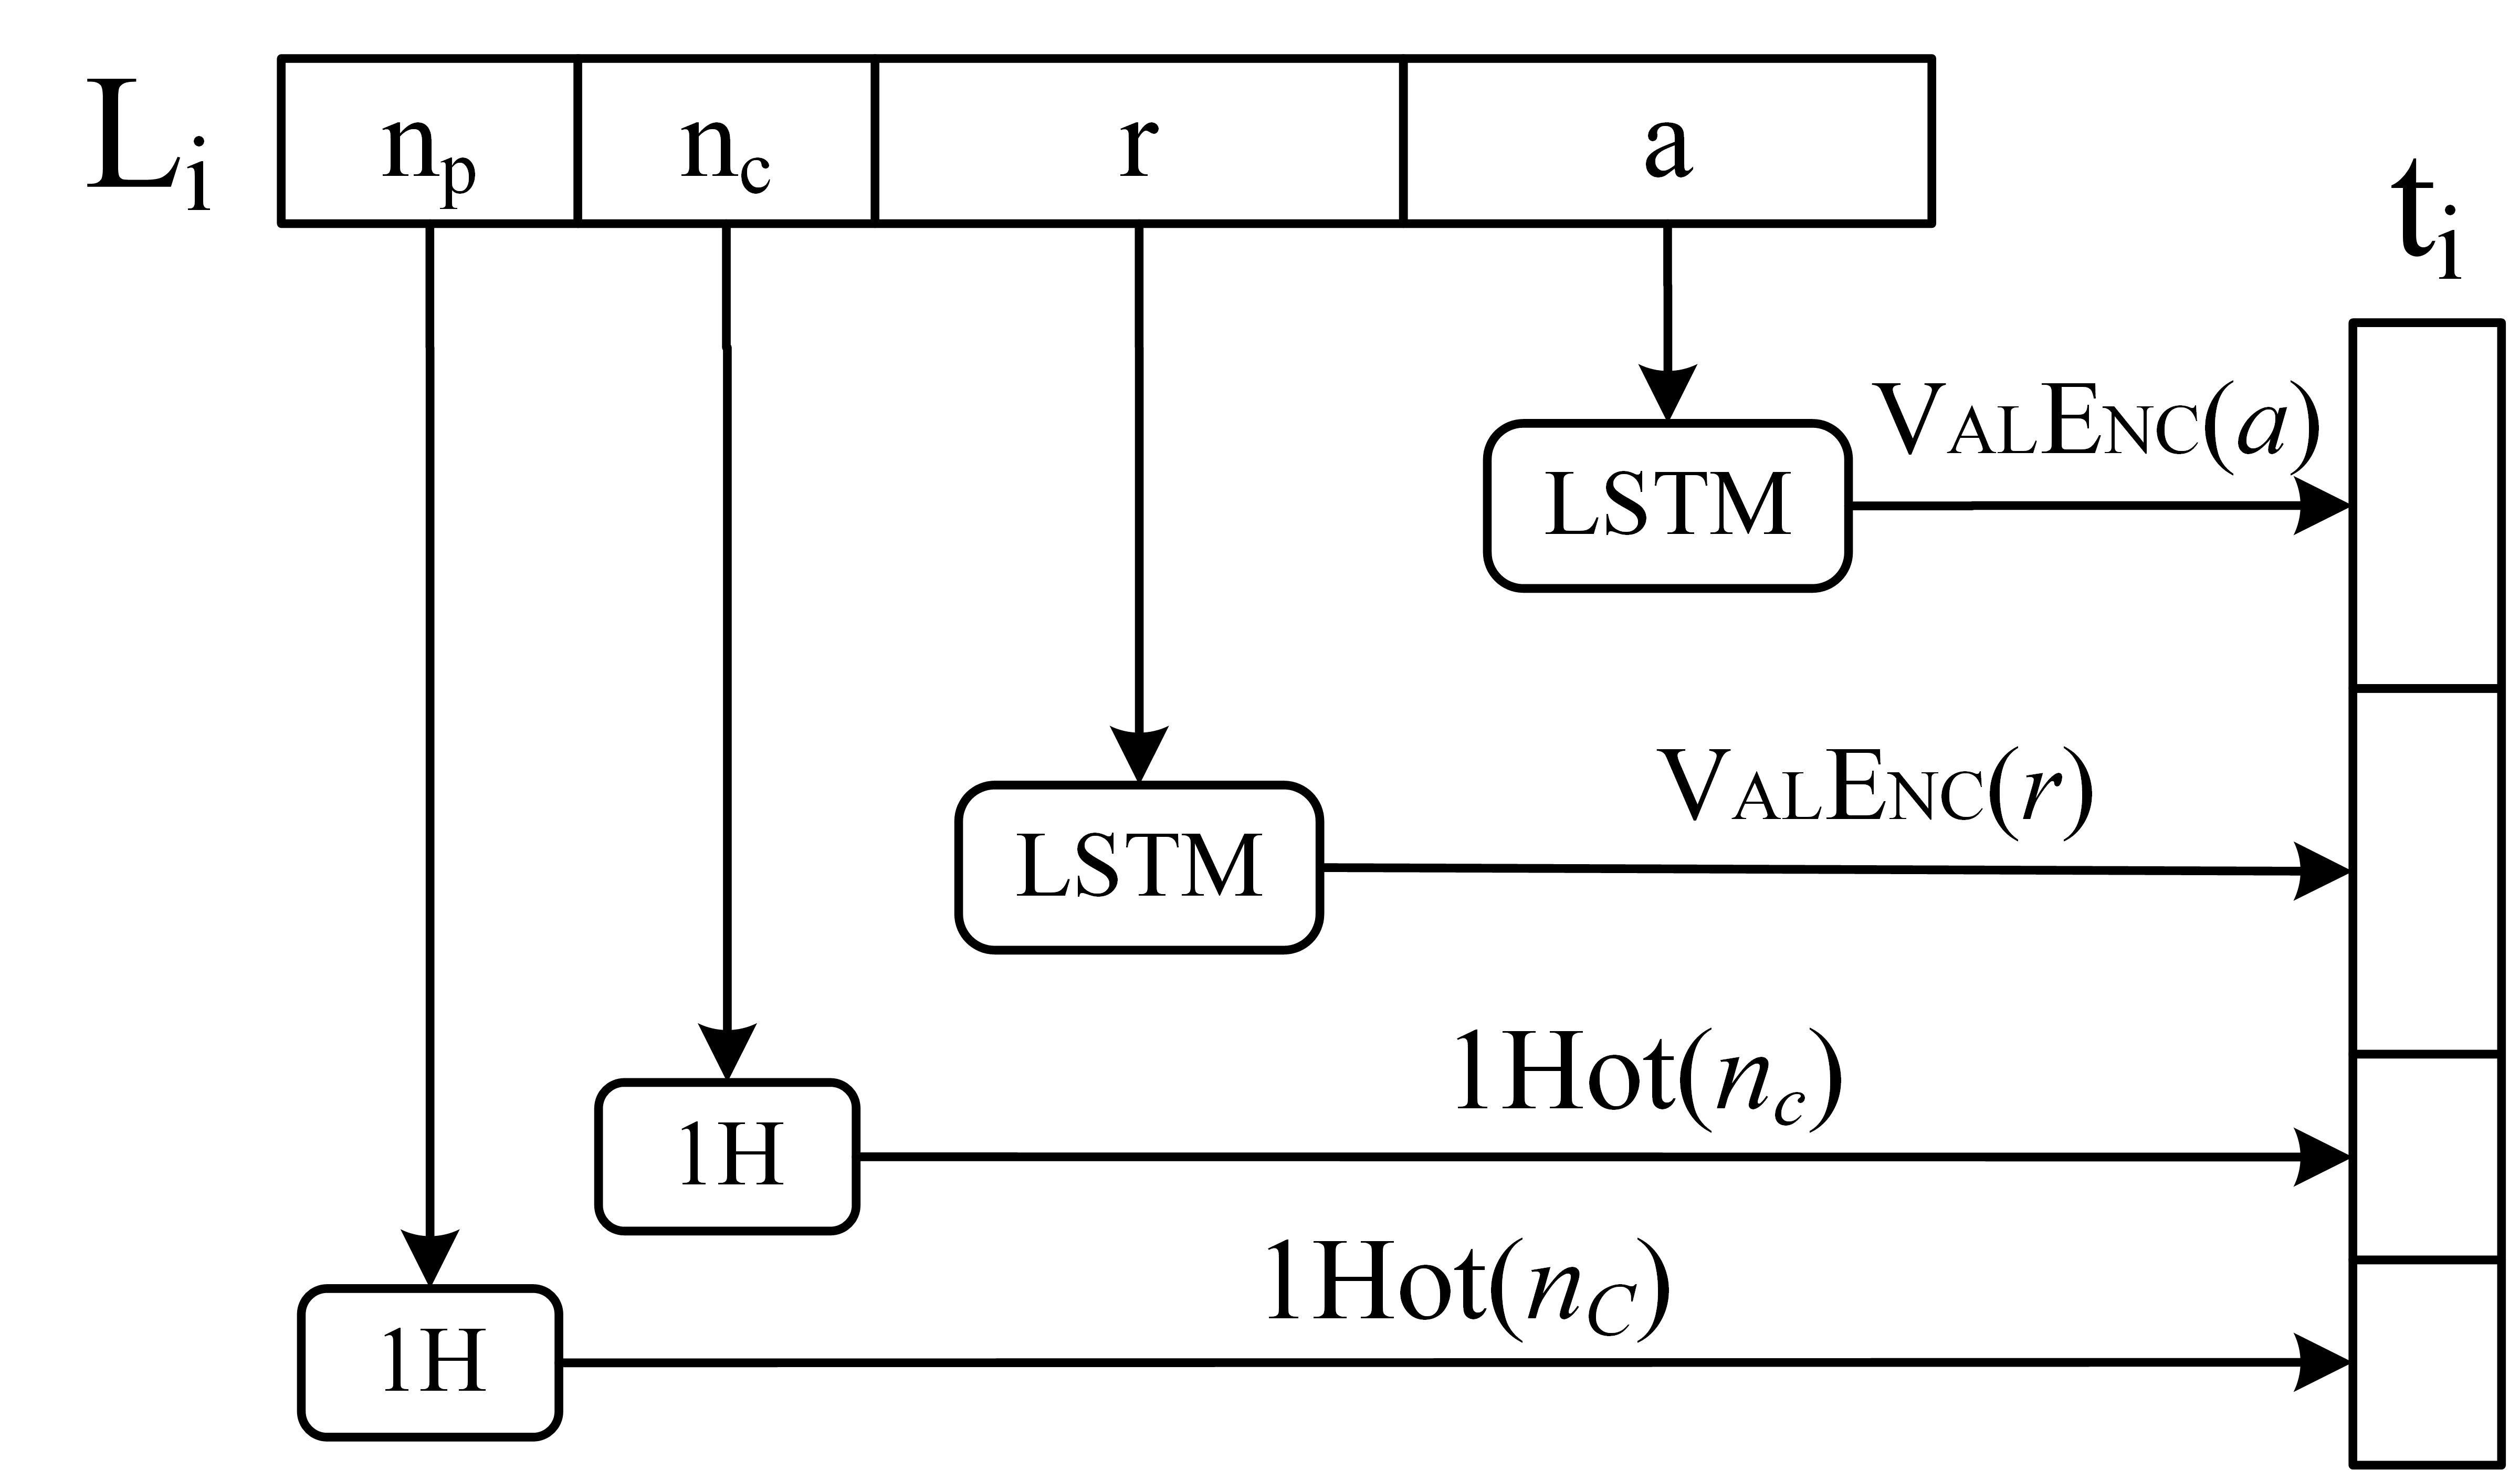
\includegraphics[scale=0.8]{../../figures/encoder_1.png} %1.0
%        \vspace{0.25cm}
%\vspace{10pt}
        \caption{\texttt{Encoder 1} representing a single line in a trace as a vector containing function caller, callee names, arguments and return values. }
%        \vspace{0.25cm}
        \label{fig:encoder-1}
    \end{subfigure}
 \vspace{-10pt}
 \caption{High-level architecture of our approach and \texttt{Encoder 1} description.}
    \vspace{-4pt}
%    \Description[High-level architecture of our approach and \texttt{Encoder 1} description.]{}
\end{figure*}
\iffalse
\begin{figure}[ht!]
    \centering
    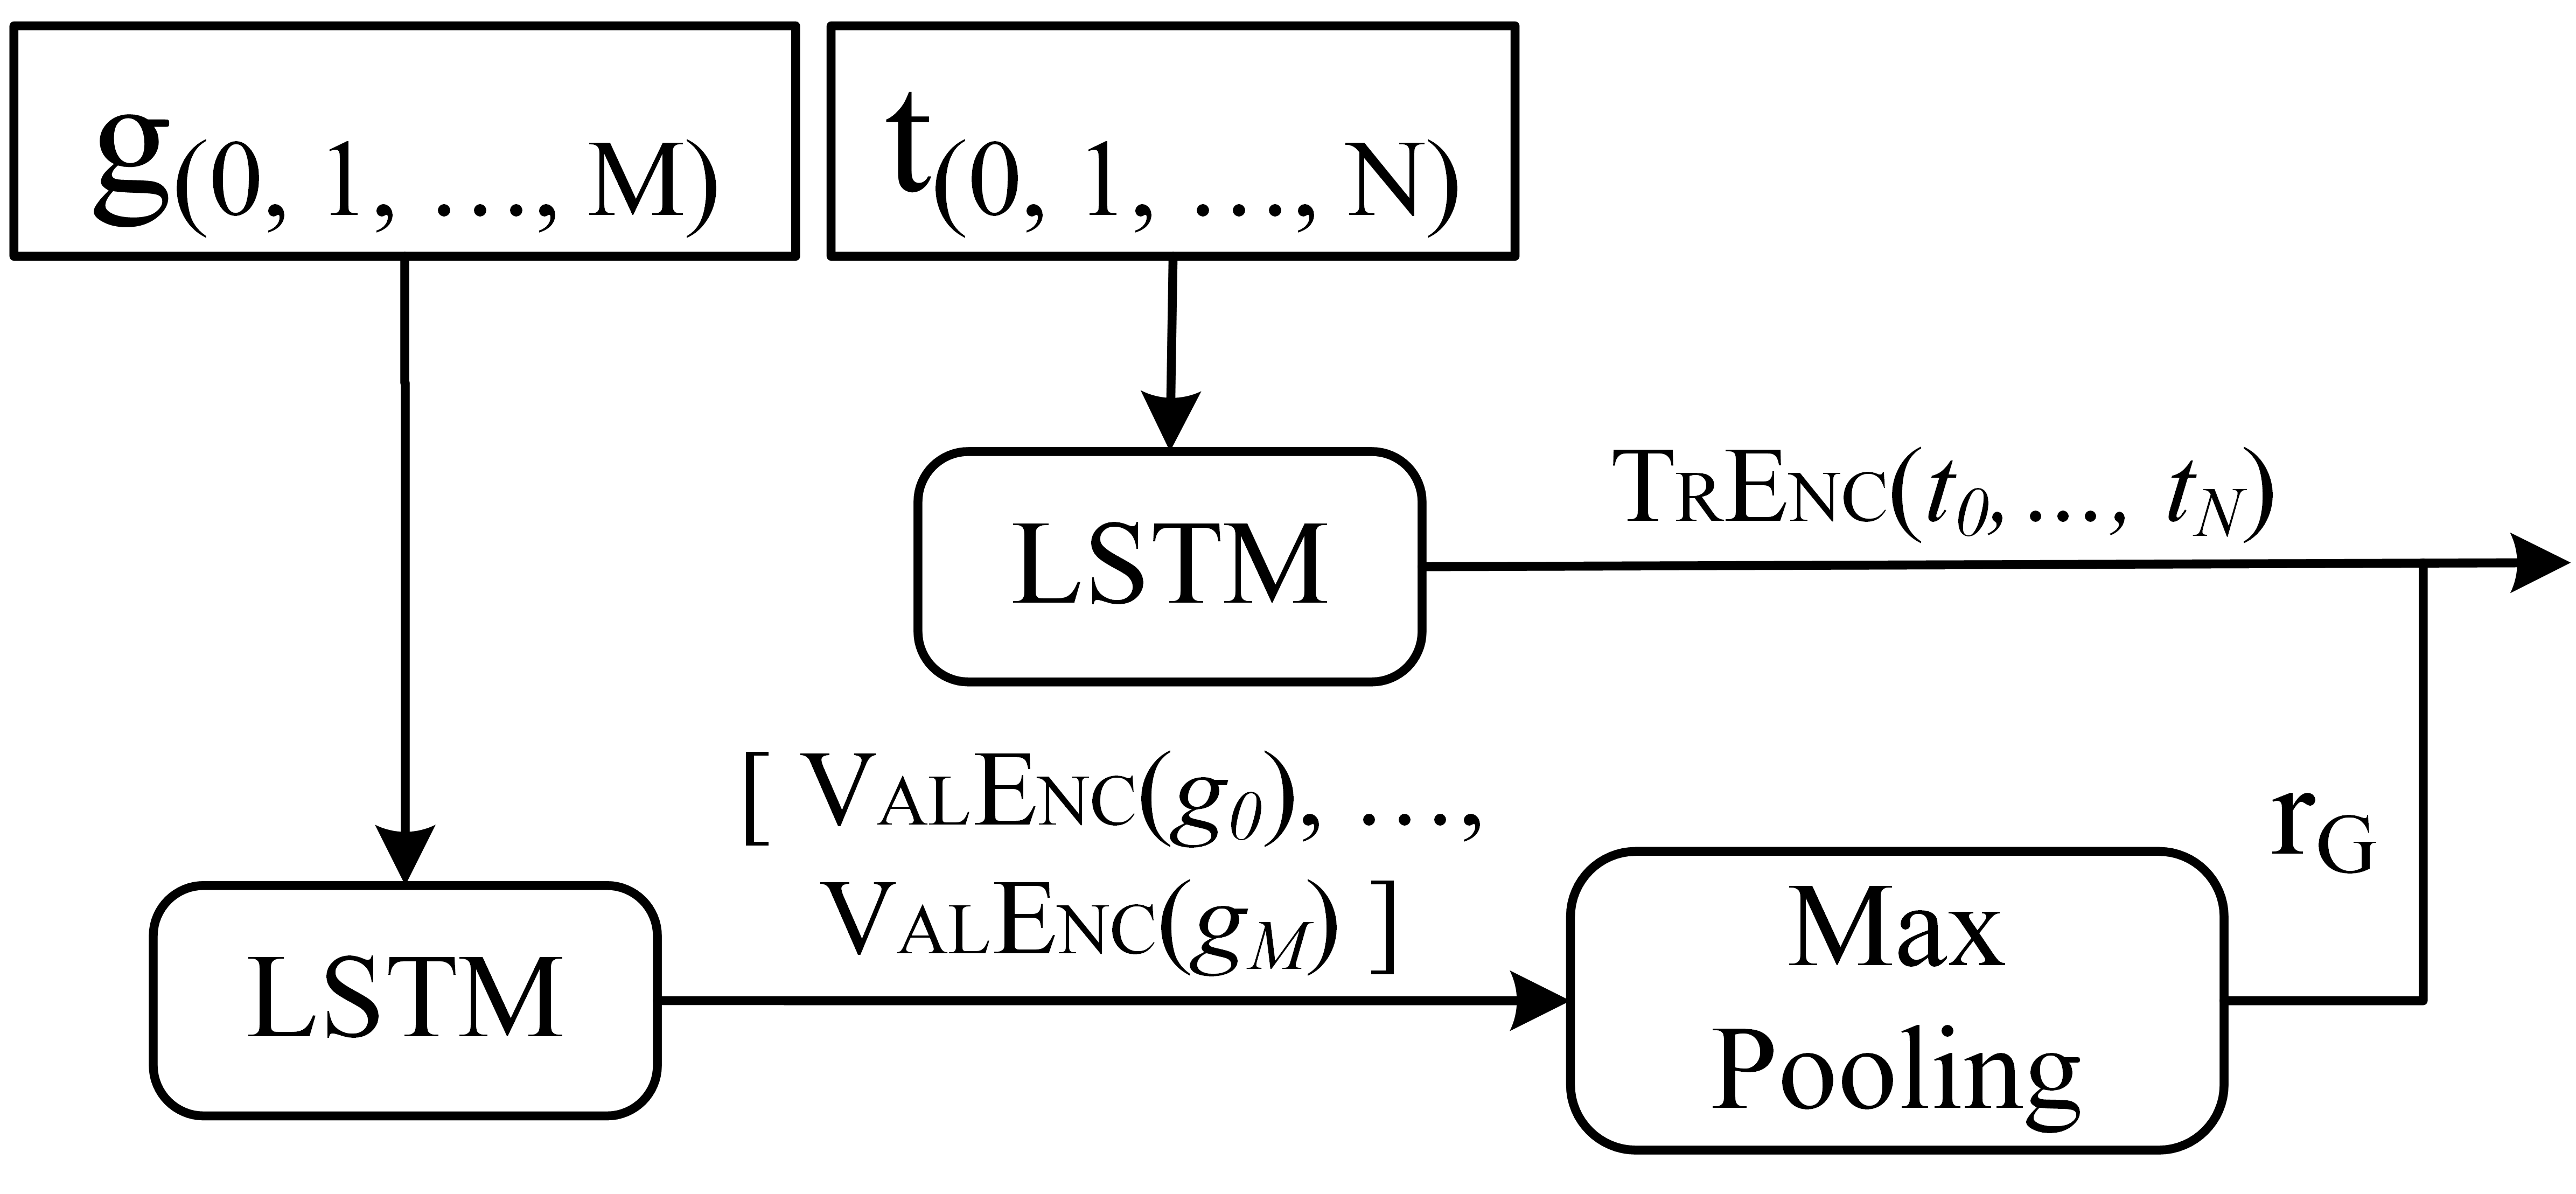
\includegraphics[scale=0.8]{../figures/encoder_2.png}
    \caption{\texttt{Encoder 2} representing a sequence of trace lines and global state as a single vector.}
    %\vspace{-20pt}
    \label{fig:encoder-2}
    \vspace{-10pt}
    %\Description[\texttt{Encoder 2} representing a sequence of trace lines and global state as a single vector.]
\end{figure}
\fi
\iffalse
\begin{figure}[ht!]
	\centering
	\includegraphics[scale=0.3]{../figures/mutation.png}
	\caption{Labelling test executions by matching actual and expected behavior.}
	%\vspace{-20pt}
	\label{fig:labelling}
	\vspace{-10pt}
	%\Description[\texttt{Encoder 2} representing a sequence of trace lines and global state as a single vector.]
\end{figure}
\fi
Our approach for building an automated test oracle for classifying execution traces has the following steps,
\begin{description}[itemsep = 0pt, topsep = 0pt, partopsep=0pt]
 \item[Step 1:] Instrument the PUT to gather traces when executing the test inputs.
 \item[Step 2:] Preprocess the traces to prune unnecessary information.
 \item[Step 3:] Encode the preprocessed traces into vectors that can be accepted by the neural network.
 \item[Step 4:] Design a NN model that takes as input an encoded trace, and outputs a verdict of pass or fail for that trace.
\end{description}
Figure~\ref{fig:pipeline} illustrates the steps in our approach, with the bottom half of the figure depicting steps 3 and 4 for any given preprocessed trace from step 2.
We discuss each of the steps in the rest of this Section.
%A high level view of our system is shown in figure~\ref{fig:pipeline}.
% \begin{itemize}
% \item The runtime instrumentation framework.
% \item The data preprocessing tool.
% \item The encoding of the traces.
% \item The architecture of the neural network.
% \end{itemize}

\subsection{Instrument and Gather Traces}
\label{sec:instrument}
For every test input executed through the PUT, we aim to collect an execution trace as a sequence of method invocations, where we capture the name of the method being called, values and data types of parameters, return values and their types, and, finally, the name of the parent method in the call graph. We find gathering further information, eg. updates to local variables within each method, incurs a significant overhead and is difficult to scale to large programs. %information in traces incurs a significant overhead for large programs.
To gather this information we use the middleware of LLVM~\cite{LLVMoriginal} and instrument the intermediate representation (IR) of programs.
This allows our implementation to be language-agnostic. LLVM provides front-end support for multiple programming languages, such as C/C++, CUDA, Haskell, Swift, Rust among others, along with numerous libraries for optimisation and code generation.
%\item The IR provides a detailed, but high-level, view of the program interactions with the memory and data type initialization, thus potentially exposing information about defects that would not be easily observed in the high-level code.
%\item The high-level constructs and features of the programming language are simplified and unified, removing syntactic sugar that induces unneeded sparsity to the data
%while allowing us to instrument these programs more easily.


% TODO: Find better symbols!
\newcommand{\callerName}{\ensuremath{n_p}\xspace}
\newcommand{\calleeName}{\ensuremath{n_c}\xspace}
\newcommand{\rVal}{\ensuremath{r}\xspace}
\newcommand{\argVals}{\ensuremath{a}\xspace}
%\ajitha{2 sentences on LLVM IR ..}
To perform the instrumentation, we traverse the PUT, visiting each method. Every time a method invocation is identified, code is injected to trace the caller-callee pair, the arguments and the return values. At the end of the program, code is inserted to write the trace information to the output.

Each trace contains a sequence of method invocations. This sequence comprises multiple lines, each line being a tuple $(\callerName, \calleeName, \rVal, \argVals)$ that represents a single method invocation within it having:

\begin{itemize}
\item The names of the caller (parent) \callerName and called \calleeName functions.
\item Return values \rVal of the call, if any.%\ajitha{Types?? After bullets}
\item Arguments passed \argVals, if any.
\end{itemize}
The order of trace lines or method invocations is the order in which the methods complete and return to the calling point. We support all variable types including primitive types (such as \texttt{int, float, char, bool}), composite data types (such as structs, classes, arrays) defined by a user or library,  and pointers for return and argument values. Structs and classes are associated with a sequence of values for their internal fields. We instrument these data structures in a depth first fashion, until all primitive types are traced. For pointers, we monitor the values they refer to.  %\foivos{anything special for recording values of pointers?}


%\textcolor{blue}{The types of the return and argument values can be a primitive, user or library-defined types in the high-level source code. As for class objects, they are represented as a sequence of their %underlying primitive fields. This happens by instrumenting fields in a DFS manner, until all primitive types are traced.}

%\ajitha{How is global state represented within the trace? Below}

%\textcolor{blue}{Within the second section of the trace, each line contains the value of one global variable before program termination. This line might contain a single number (if the respective variable is a primitive type), or a sequence of values (if the variable is a class object with multiple internal fields). }

\subsection{Training Set}
\label{sec:labelled-traces}
We execute the instrumented program with each test input in the test suite to gather a set of traces. A subset of the traces is labelled and used in training the classification model. To label the traces as pass or fail, we compare actual outputs through the PUT with expected outputs provided by a reference program or the specifications. %, as shown in figure~\ref{fig:labelling}.
Section~\ref{sec:labelling-traces} discusses how we label traces for the subject programs in our experiment. 
It is worth noting that in our approach, the developer will only need to provide expected outputs for a \emph{small proportion of tests rather than the whole test suite}. %In current practices, the developer or tester provides expected outputs for the whole test suite which is considerably more effort than the 15\% we require. 
In the absence of expected output in tests, how will tests be labelled is a common question. Answering this question will depend on what is currently being done by the developer or organisation for classifying tests as pass or fail. Our approach will entail applying the same practice to labelling, albeit to a significantly smaller proportion of tests.    % will rely on the existing test classification practice used by the organisation to label a small proportion of tests.
%The advantage with our technique is that only a small proportion of the traces will need to be labelled as opposed to all the tests which is the case for current practices.
%
%If the tests do not specify expected outputs, then the relevant technique that the develper or organisation currently relies on for classifying tests can be used to label the traces. This relevant technique may be manual inspection, a golden reference model or a developer or expert would have to manually label the traces used in training, which is a small proportion of the total traces.  Reuiring a small proportion of traces to be labelled is \emph{not} a limitation of our approach
\iffalse
\textcolor{red}{We also find that some programs are only accompanied by passing tests, whereas both classes} are needed in the training set.
To generate failing tests, we keep the original program as a reference for the expected outputs and we use common bugs to mutate it. If a test's output deviates from the expected output, it is labelled as failing, otherwise passing. We gather all execution traces by running all tests through the mutated program.
We apply the following mutations representing some common bug patterns~\cite{jia2011analysis, pradel2018deepbugs}: %that are most applicable to the code structure and syntax for the subject programs in our experiment:
\begin{enumerate}[itemsep = 0pt, topsep = 0pt, partopsep=0pt]
	\item Logical connector replacement applied to \{$\&\&, ||, !$\}.
	\item Relational operator replacement applied to \\ \{$<, > , ==, <=, >=, !=$\}.
	\item Argument swapping in function calls.
	\item Scalar variable replacement.
	\item Loop boundary value replacement.
\end{enumerate}
\fi
To avoid data leakage in our experiment in Section~\ref{sec:experiment}, we ensure that expected output is removed from the traces. We also remove exceptions, assertions and any other information in the program or test code that may act as a test oracle. This is further discussed in Section~\ref{sec:subj-programs}. %\foivos{This is what we originally mentioned for data leakage}
%
%We assume that the original program is correct and, therefore, the traces gathered from it are labeled as passing. To produce failing traces, random mutations are applied to the %original IR of the program. In this work, we consider swapping binary operators, changing loop boundaries, inverting Boolean statements or swapping the arguments in a function %call. Each mutation generates a single set of failing traces.
%
%Even though the test cases of the projects we study, are using assertions to compare the computed with the expected output
%The test cases of the projects we study, are using assertions to compare the computed with the expected output of each test input. However, it is important to note that, before instrumentation, we have removed these assertions or any other kind of information that could betray the validity of the output. The desired behavior of our architecture is to understand how the control flow is correlated with the input, output and the correctness of a program, instead of overfitting on a binary state, which is at the end of the trace and represents if the test passed or failed.

\subsection{Preprocessing}
The execution traces gathered with our approach include information on methods declared in external libraries, called during the linking phase. To keep the length of the traces tractable and relevant, we preprocess the traces to only keep trace lines for methods that are defined within the module, and remove trace lines for declared functions that are not defined, but simply linked to later.
%to only keep trace lines for methods and implementations defined by the \textcolor{red}{user} \foivos{user defined methods are a subset of the defined functions in a IR module. Others are functions from locally-based header files included, or methods not explicitly specified by the user, e.g. constructors for the containers they use. They are as well important} and remove
%trace lines for declared functions from external libraries.
%The execution traces collected can be quite long. Due to well-known limitations of neural networks with long sequences, it is necessary to preprocess the traces to reduce their length. The length of the traces is large, predominantly due to the fact that, on compiler level, many function are invoked to construct objects at the beginning of each program. For example, invoking a simple C++ function that only initializes and returns a vector, can produce an execution trace of 50 lines. To alleviate this issue, function calls that occur before a certain point in the trace are rejected. We choose that point to be the first function call that directs the control flow to the function (or the first function among many) under test \foivos{this sentence is too cryptic!}. This approach is correct since before reaching the tested function, no differences relative to potential bugs can be observed.
%\foivos{The above paragraph is very hard to understand, what are you trying to say? What trace lines are disregarded?}

For method invocations within loops, a new trace line is created for each invocation of the same method within the loop. For loops with large numbers of iterations, this can lead to redundancy when the method is invoked with similar arguments and return values. We address this potential redundancy issue by applying average pooling to trace lines with identical caller-callee methods within loops.
%Furthermore, function calls inside lengthy loops can lead to an unwanted increase of trace length. In most cases, functions called inside loops receive similar arguments and return similar values. To summarize information from identical function calls in a sequence, average pooling is applied to these lines. If the number of consecutive identical sequences of function calls surpass a threshold, then pooling is applied to this sequence. As an example, if 50 sequential function calls with identical sets of caller-callee functions are found into a trace, they will be summarized as 10 averaged lines by selecting pooling kernel and stride equal to 5, if pooling is activated. Selecting the length of the pooling kernel, as well as the threshold which triggers it, is specified individually for each application, after experimenting with the original traces.


% excluded declared functions which are typically called during the linking phase. These declared functions are external library functions, like methods for STL containers and functions in the BOOST library.
%- why?
% Too expensive to monitor everything, menanigful information will be lost, you assume library functions work correctly
% only trace method invocations that are defined and implemented within the PUT.
%\foivos{I have my doubts about the former paragraph. We might create more questions than explain something actually meaningful. Also it is not that this pooling is so important to the preprocessing. It is rather used in 1-2 occasions}

 % \foivos{What is avg pooling in this setting?} \miltos{Well, the idea is: If you have a function call inside a loop, then you will find in the trace, X consecutive lines being exactly the same, or almost the same, differing just a bit in their arguments (most of the times because of loop increment). So, for example, if the preprocessor found 50 consecutive function calls, with the same caller-callee pair, it would apply avg pooling with kernel=stride= say 10, and you would end up with 5 averaged lines, instead of 50.} \foivos{Then explain this in the text and delete these TODOs}

\subsection{Neural Network Model}
\label{sec:NN-model}
\newcommand{\valEncoder}{\textsc{ValEnc}\xspace}
\newcommand{\traceEncoder}{\textsc{TrEnc}\xspace}
\newcommand{\traceClassifier}{\textsc{TraceClassifier}\xspace}
In this step, we perform the crucial task of designing a neural network that learns to classify the pre-processed traces as passing or failing.
Shape and size of the input traces vary widely, and this presents a challenge when designing a NN that accepts fixed length vectors summarizing the traces.
%The challenge arises from the widely varying shape and size of the input traces. Although this is a standard classification problem, the shape and size of each trace differs widely.
To address this, our network comprises three components that are trained jointly and end-to-end: 1. a \valEncoder that encodes values (such as the values of arguments and return values) into $D_V$-dimensional distributed vector representations, shown within \texttt{Encoder 1} in Figure~\ref{fig:encoder-1}, 2. a \traceEncoder that encodes variable-sized traces into a single $D_T$-dimensional vector, shown as \texttt{LSTM} in Figure~\ref{fig:pipeline}, and finally, 3. a \traceClassifier that accepts the trace representation for state and predicts whether the trace is passing or failing. The \texttt{Multi-layer Perceptron} in Figure~\ref{fig:pipeline} represents the \traceClassifier.  We describe each component in detail in the rest of this section.

\textbf{Encoding Values}
Values within the trace provide useful indications about classifying a trace. % and therefore, we need to incorporate information about those values in a way that our neural network can learn from patterns within them.
However, values --- such as ints, structs, and floats --- vary widely in shape and size. We, therefore, design models that can summarize variable-sized sequences into fixed-length representations. In the machine learning literature, we predominantly find three kinds of models that can achieve this: recurrent neural networks (RNNs), 1D convolutional neural networks (CNN) and transformers. In this work, we employ LSTMs~\cite{hochreiter1997long} --- a commonly used flavour of RNNs. Testing other models is left as future work. At a high-level RNNs are recurrent functions that accept a vector $\mathbf{h}_t$ of the current state and an input vector $\mathbf{x}_t$ and compute a new state vector $\mathbf{h}_{t+1}=RNN(\mathbf{x}_t, \mathbf{h}_t)$ which ``summarizes'' the sequence of inputs up to time $t$. A special initial state $\mathbf{h}_0$ is used at $t=0$.

To encode a value $v$, we decompose it into a sequence of primitives $v=[p_0, p_1, ...]$ (integers, floats, characters, etc.). Each primitive $p_i$ is then represented as a binary vector $\mathbf{b}_i=e(p_i)$ containing its bit representation padded to the largest primitive data type of the task. For example, if \texttt{int64} is the largest primitive then all $\mathbf{b}_i$s have dimensionality of 64. This allows us to represent all values (integers, floats, strings, structs, pointers, etc.) as a unified sequence of binary vectors. We encode $v$ into a $D_V$-dimensional vector by computing
\begin{align*}
	\valEncoder(v) = LSTM_{v}(e(p_L)_L, \valEncoder([p_0, p_1, ..., p_{L-1}])),
\end{align*}
where $LSTM_{v}$ is the LSTM that sequentially encodes the $\mathbf{b}_i$s. Note that we use the same \valEncoder for encoding arguments and return values, as seen in Figure~\ref{fig:encoder-1}. The intuition behind this approach is that the bits of each primitive can contain valuable information. For example, the bits corresponding to the exponent range of a float can provide information about the order of magnitude of the represented number, which in turn may be able to discriminate between passing and failing traces.

\textbf{Representing a Single Trace Line}
\newcommand{\OneHot}{\textsc{1Hot}\xspace}
Armed with a neural network component that encodes values, we can now represent a single line $(\callerName, \calleeName, \rVal, \argVals)$ of the trace. To do this, we use \valEncoder to encode the arguments \argVals and the return value \rVal. We concatenate these representations along with one-hot representations of the caller and callee identities, as shown in Figure~\ref{fig:encoder-1}. Specifically,
the vector encoding $\mathbf{t_i}$ of the $i$th trace line is the concatenation
\begin{align*}
	\mathbf{t_i} = \left[ \valEncoder(\argVals), \valEncoder(\rVal), \OneHot(\callerName), \OneHot(\calleeName) \right],
\end{align*}
where \OneHot is a function that takes as input the names of the parent or called methods and returns a one-hot vector that uniquely encodes that method name. For methods that are rare (appear fewer than $k_{min}$ times) in our data, \OneHot collapses them to a single special Unknown (UNK) name. This is similar to other machine learning and natural language processing models and reduces sparsity often improving generalization.
The resulting vector $\mathbf{t_i}$ has size $2D_V+2k$ where $k$ is the size of each one-hot vector.

\textbf{Encoding Traces}
Now that we have built a neural network component that encodes single lines within a trace, we design \traceEncoder that accepts a sequence of trace line representations $\mathbf{t}_0 ... \mathbf{t}_N$ and summarizes them into a single $D_T$-dimensional vector. We use an LSTM with a hidden size $D_T$, and thus
\begin{align*}
	\traceEncoder(\mathbf{t}_0 ... \mathbf{t}_N) = LSTM_{tr}\left(\mathbf{t_N}, \traceEncoder(\mathbf{t}_0 ... \mathbf{t}_{N-1}) \right),
\end{align*}
where $LSTM_{tr}()$ is an LSTM network that summarizes the trace line representations. %Figure~\ref{fig:encoder-2} shows \traceEncoder along with global state encoding.

\iffalse
\textcolor{red}{\textbf{Encoding Global State} We encode the final values of global variables in each trace. %The global state can provide valuable information for trace classification and thus we also encode the values within the global state.
Assuming global variables $g_0, ..., g_M$, we first encode them using \valEncoder and then summarize the global state into a single vector
\begin{align*}
\mathbf{r}_G = \textsc{Pool}(\valEncoder(g_0), ... \valEncoder(g_M)),
\end{align*}
where \textsc{Pool} is a permutation-invariant pooling function and $\mathbf{r}_G$ is a $D_V$-sized vector. In this work, we use max pooling (i.e. element-wise maximum). Note that the permutation invariance is a necessary design requirement since the representation of the global state should be invariant to the ordering of the global variables. Figure~\ref{fig:encoder-2} shows \traceEncoder along with global state encoding.}
\fi

\textbf{Classifying Traces}
%Our task is to classify a trace into either passing or failing.
With the neural network components described so far we have managed to encode traces into fixed length vector representations. The final step is to use those computed representations to make a classification decision. We treat failing traces as the positive class and passing traces as the negative class since detecting failing runs is of more interest in testing.  We compute the probability that a trace is failing as
\begin{align*}
	P(\textsf{fail}) = \traceClassifier([\traceEncoder(\mathbf{t}_0 ... \mathbf{t}_N)]),
\end{align*}
where the input of \traceClassifier is the output vector of \traceEncoder. Our implementation of \traceClassifier is a multilayer perceptron (MLP) with sigmoid non-linearities and a single output, which can be viewed as the probability that the trace is a failing trace. It follows that $P(\textsf{pass})=1-P(\textsf{fail})$.

\textbf{Training and Implementation Details}
We train our network end-to-end in a supervised fashion, minimizing the binary cross entropy loss. All network parameters (parameters of $LSTM_v$ and $LSTM_{tr}$ and parameters of the MLP) are initialized with random noise.
For all the runs on our network we use $D_V=128$, $D_T=256$. The \traceClassifier is an MLP with 3 hidden layers of size 256, 128 and 64.
We use the Adam optimizer~\cite{AdamOptimizer} with a learning rate of $10e-5$. 

For our subject programs, we find the aforementioned feature values to be optimal for performance and training time, after having experimented with other NN architectures, varying the $D_V$, $D_T$ sizes, and the hidden layers in the MLP. We explored increasing $D_V$ to 256, 512, $D_T$ to 512, 1024 and size of hidden layers to 512 and 1024.

To handle class imbalance in datasets, 
%Since the failing/passing trace dataset has a class imbalance,
we explicitly counteract the imbalance in the loss function by down-weighting the samples within the most popular class such that samples of both
class participate equally within this function.
%\foivos{Feature sizes tried and what was chosen for the different subject programs.} \ajitha{Ok, done, check below and delete todo. I think I wrote too many things and maybe some of them could belong to experiment section rather than here.}

Our implementation of the proposed approach is available at \emph{\url{https://github.com/fivosts/Learning-over-test-executions}. }

%We have uploaded the source code of our approach to a public anonymous repository\footnote{\url{https://github.com/anon-0/ASE-ClassifyTestExec}}, the link of which is provided.

%%We found increasing each of these features did not improve performance or the convergence rate.
%%This proposed architecture, the feature sizes and the optimizer were selected after experimenting on the evaluated case studies. We trained our model by combining a set of different values for  $D_V$, $D_T$ and the hidden layers of the MLP. By increasing $D_V$ to 128, 256, 512 and $D_T$ to 256, 512, 1024 the model neither achieves better performance nor does it converge faster than with the proposed feature sizes. The same conclusion applies to increasing the hidden layers of the MLP up to 1024, 512 and 256 respectively. However, the computational complexity of the training phase increases dramatically.
%%Decreasing the feature sizes below the proposed values results in reduced precision and recall. Reducing the hidden size of the LSTM encoders for the arguments and return values, significantly affects the performance for subject programs that have structs or classes as arguments or return values since a small encoder is inadequate in summarizing the information from these data structures.
%%does not affect the case studies that use mostly primitive types as arguments and return values.
%%However, the subject programs, in which structs or classes appear as arguments or return values, were significantly affected. This is because classes contain multiple fields, all of which are monitored. As a result, the sections that contain these data types are very large and a smaller encoder is incapable of extracting its features.
%%Reducing the size of the hidden layers of the MLP also affects precision and recall, becoming biased towards a ``pass" or ``fail" classification.
%%In this case, we noticed that the network is not able to perform well in both output classes, becoming biased towards ``pass" or ``fail" classification, especially in programs where wrong behavior might be implied by a wider range of different patterns. Furthermore, we noticed that reducing the number of the hidden layers by one, it cannot perform well, despite increasing the size of the two remaining layers.
%%\miltos{Check if this paragraph about other feature sizes is worth mentioning}


\section{Experiment}
 \label{sec:experiment}
In our experiment, we evaluate the feasibility and accuracy of the NN architecture proposed in Section~\ref{sec:approach} to classify execution traces for 4 subject programs and their associated test suites.
We investigate the following questions regarding feasibility and effectiveness:
%\begin{description}[itemsep = 0pt, topsep = 0pt, partopsep=0pt]
%\item[Q1. Precision, Recall and Specificity:] 
%\textit{What is the precision, recall and specificity achieved over the subject programs? }
%
%To answer this question, we use our tool to instrument the source code to 
%record execution traces as sequences of method invocations, arguments and return values. 
%%\foivos{As the NN architecture have already been decided and we do not want to tune its hyperparameters, the data are not divided into a training, validation and testing set}. 
%A small fraction of the  execution traces are labelled (\emph{training set}) and fed to our framework to infer a classification model. We then evaluate precision, recall and specificity achieved by the model over unseen execution traces (\emph{test set}) for that program. The test set includes both passing and failing test executions. We use \emph{Monte Carlo cross-validation}, creating random splits of the dataset into training and test data. We created 15 such random splits and averaged precision, recall and specificity computed over them. In our experiments, we do not use a validation set to tune the hyper-parameters in the NN model.  
%%Additionally, we check if the inferred model can detect bug patterns in the test set that were unseen in the training set.  
%%in include failing instances from some The unseen test executions include failing instances from common bug patterns in programs. 
%%Instead, we divide them into a training and an evaluation set. We calculate the model's performance on the evaluation set.
%
%\item[Q2. Size of training set:] 
%\textit{How does size of the training set affect precision and recall of the classification model?}
%
%For each program, we vary the size of training set from 5\% to 30\% of the overall execution traces and observe its effect on precision and recall achieved. 
%
%\item[Q3. Comparison against state of art:]
%\textit{How does the precision, recall and specificity achieved by our technique compare against agglomerative hierarchical clustering, proposed by Almaghairbe et al.~\cite{almaghairbe2017separating} in 2017? }
%
%We choose to compare against the hierarchical clustering work as it is the most relevant and recent in classifying execution traces. Traces used in their work are sequences of method invocations, similar to our approach. Other test oracle work that use NNs is not used in the comparison as they do not work over execution traces, and are limited in their applicability to programs with numerical input and output which is not the case for programs in our experiment. 
%\iffalse
%\textcolor{red}{\item[Q4. Generalisation of classification model: ]
%\textit{Can a classification model inferred from a program in a particular application domain be used to classify test executions over other programs in the same domain?}
%\\
%For the network protocol domain, we evaluate the accuracy of using a classification model inferred using traces from a single protocol detection finite state machine (FSM) for classifying test executions from other protocol FSMs. }
%\fi
%\end{description}


\textbf{Q1. Precision, Recall and Specificity:} 
\textit{What is the precision, recall and specificity achieved over the subject programs? }

To answer this question, we use our tool to instrument the source code to 
record execution traces as sequences of method invocations, arguments and return values. 
%\foivos{As the NN architecture have already been decided and we do not want to tune its hyperparameters, the data are not divided into a training, validation and testing set}. 
A small fraction of the  execution traces are labelled (\emph{training set}) and fed to our framework to infer a classification model. We then evaluate precision, recall and specificity achieved by the model over unseen execution traces (\emph{test set}) for that program. The test set includes both passing and failing test executions. We use \emph{Monte Carlo cross-validation}, creating random splits of the dataset into training and test data. We created 15 such random splits and averaged precision, recall and specificity computed over them. In our experiments, we do not use a validation set to tune the hyper-parameters in the NN model.  
%Additionally, we check if the inferred model can detect bug patterns in the test set that were unseen in the training set.  
%in include failing instances from some The unseen test executions include failing instances from common bug patterns in programs. 
%Instead, we divide them into a training and an evaluation set. We calculate the model's performance on the evaluation set.

\textbf{Q2. Size of training set:}
\textit{How does size of the training set affect precision and recall of the classification model?}

For each program, we vary the size of training set from 5\% to 30\% of the overall execution traces and observe its effect on precision and recall achieved. 

\textbf{Q3. Comparison against state of art:}
\textit{How does the precision, recall and specificity achieved by our technique compare against agglomerative hierarchical clustering, proposed by Almaghairbe et al.~\cite{almaghairbe2017separating} in 2017? }

We choose to compare against the hierarchical clustering work as it is the most relevant and recent in classifying execution traces. Traces used in their work are sequences of method invocations, similar to our approach. Other test oracle work that use NNs is not used in the comparison as they do not work over execution traces, and are limited in their applicability to programs with numerical input and output which is not the case for programs in our experiment. 


All experiments are performed on a single machine with 4 Intel i5-6500 CPU cores, Nvidia RTX 2060 GPU, 16GB of memory. %No dedicated GPU was used to any part of the experiment (instrumentation, training or testing).


\subsection{Labelling Traces}
\label{sec:labelling-traces}
%We chose subject programs from different domains to assess applicability of our approach, namely from the blockchain, deep learning, encryption and text editing domains. 
All our subject programs are open source, and most of them were only accompanied by passing tests. This is not uncommmon as most released versions of programs are correct for the given tests. We take these correct programs to be reference implementations. To enable evaluation of our approach that distinguishes correct versus incorrect executions, we need subject programs with bugs. We, therefore, generate PUTs by automatically mutating the reference implementation using common mutation operators~\cite{jia2011analysis} listed below, 
\begin{enumerate}[itemsep = 0pt, topsep = 0pt, partopsep=0pt]
	\item {Arithmetic operator replacement applied to \{$+, -, *, /,\\ --, ++$\}.}
	\item {Logical connector replacement applied to \{$\&\&, ||, !$\}.}
	\item {Bitwise operator replacement applied to \{$\&, |, \wedge, ~, <<, >>$\}.}	\item {Assignment operator replacement applied to \\ \{$+=, -=, *=, /=, \%=, <<=, >>=, \&=, |=, \wedge=$\}.}
\end{enumerate}
\begin{figure}[ht!]
	\vspace{-12pt}	
	\centering
	\includegraphics[scale=0.3]{../../figures/mutation.png}
	\caption{Labelling test executions by matching actual and expected behavior.}
	%\vspace{-20pt}
	\label{fig:labelling}
	\vspace{-10pt}
	%\Description[\texttt{Encoder 2} representing a sequence of trace lines and global state as a single vector.]
\end{figure}
A PUT is generated by seeding a single fault into the reference implementation at a random location using one of the above mutation operators. 
We used an independent open source mutation tool\footnote{\url{https://github.com/chao-peng/mutec}} to generate PUTs from a given reference program. 
Figure~\ref{fig:labelling} shows a PUT generated by seeding a single fault into a reference program.
As seen in Figure~\ref{fig:labelling}, we run each test, $T_i$, in the test suite, through both the reference program and PUT, and label the trace as \emph{passing} if the expected output, $EO_i$, from the reference matches the actual output, $AO_i$, from the PUT. If they do not match, the trace is labelled as \emph{failing}.  
We rejected PUTs from mutations that did not result in any failing traces (outputs always match with the reference). This avoids the problem of equivalent mutants. 
All the PUTs in our experiment had both passing and failing traces. 
%To generate failing tests, we keep the original program as a reference for the expected outputs and we use common bugs to mutate it, as shown in figure~\ref{fig:labelling}. The mutated program is the SUT. If a test's output deviates from the expected output, it is labelled as failing, otherwise passing. We gather all execution traces by running all tests through the SUT.
%We apply the following mutations representing some common bug patterns~\cite{jia2011analysis, pradel2018deepbugs}: %that are most applicable to the code structure and syntax for the subject programs in our experiment:
%To avoid data leakage in our experiment, we ensure that expected output is removed from the traces. We also remove exceptions, assertions and any other information in the program or test code that may act as a test oracle. 

\subsection{Subject Programs}
\label{sec:subj-programs}
We chose subject programs from different domains to assess applicability of our approach, namely from the blockchain, deep learning, encryption and text editing domains. A description of the programs and associated tests is as follows. \\
\noindent\textbf{1. Ethereum}~\cite{ethereum} is an open-source platform based on blockchain technology, which supports smart contracts. Within it, we evaluate our approach over the \texttt{Difficulty} module that calculates the mining difficulty of a block, in relation to different versions (eras) of the cryptocurrency (Byzantium, Homestead, Constantinople etc.). The calculation is based on five fields of an \texttt{Ethereum} block, specified in the test input. 

\paragraph{Tests}

We use the default test inputs provided by Ethereum's master test suite for the \texttt{Difficulty} module. We test this module for the Byzantium era of the cryptocurrency (version 3.0). The test suite contains 2254 \emph{automatically} generated test inputs. Each test input contains one hex field for the test input of the difficulty formula and another hex field for the expected output of the program. All the test inputs provided with the module are passing tests with the actual output equal to the expected output. As a result, we use the provided module as a reference implementation. As described in Section~\ref{sec:labelling-traces}, we seed faults into the reference implementation to generate PUTs, each containing a single mutation. For the difficulty module, we generate 2 PUTs -- 1. Ethereum-SE with a seeded fault in the core functionality of the difficulty module, and 2. Ethereum-CD  with a fault seeded in one of the functions that is external to the core function but appears in the call graph of the module.  The balance between passing and failing tests varies between the two PUTs, Ethereum-CD being perfectly balanced and Ethereum-SE being slightly imbalanced (828 failing and 1426 passing tests). %Finally, expected outputs and assertions are removed from the traces, so that there is no existing test oracle information. It is worth noting that for all our subject programs, we systematically remove all forms of test oracle information (expected output, assertions, exception, etc.) prior to applying our approach. 
\iffalse
by mutating passing test inputs and checking if they cause the actual output to differ from the expected output. Inputs and code mutations that result in the actual and expected output to differ are used as failing traces.  We apply the following common types of mutations~\cite{jia2011analysis, pradel2018deepbugs} that are most applicable to the module code structure and syntax: 
\begin{enumerate}
	\item Logical connector replacement applied to \{$\&\&, ||, !$\}.
	\item Relational operator replacement applied to \\ \{$<, > , ==, <=, >=, !=$\}.
	\item Argument swapping in function calls.
	\item Scalar variable replacement.
	\item Loop boundary value replacement.
\end{enumerate}
In the experiments that evaluate the classification model, we ensure that the expected output is removed from the traces, along with any information and assertions in the code that compare it with the actual output.  
\fi

 
\noindent\textbf{2. Pytorch}~\cite{pytorch} is an optimized tensor library for deep learning, widely used in research. In our experiment, we evaluate our model over the \texttt{intrusive\_ptr} class, which implements a pointer type with an embedded reference count.
We chose this class because it had a sizeable number of tests (other modules had $<20$ published tests). 

\paragraph{Tests}
Implementation of the class is accompanied by 638 tests, all of which are passing. We, thus, use this as the reference implementation.  %{Each test checks for multiple assertions. We unroll each assertion to a single test to separate the test cases and increase the size of our samples. We end up with 638 passing tests.} 
As with \texttt{Ethereum}, we apply mutations to the \texttt{intrusive\_ptr} implementation to generate a single PUT. Upon comparison with the reference,  318 of the existing tests are labelled passing through the PUT and 320 as failing.  %We remove assertions from the test inputs to ensure that no bias is introduced to the training of our model.

\noindent\textbf{3. Microsoft SEAL}~\cite{sealcrypto} is an open-source encryption library. In our experiment, we study one component within Microsoft SEAL, the \texttt{Encryptor} module, which is accompanied by tests. This component is responsible for performing data encryption.

%\paragraph{NN Architecture} 

\paragraph{Tests}
The \texttt{Encryptor} component is accompanied by 133 tests. %{, each containing a large number of assertions. We split the assertions to one test each and end up with 133 tests. These tests cover a set of \texttt{Encryptor's} functions and therefore they can be grouped in groups with respect to the function that they test. This observation is important to know once a single mutation breaks the functionality of one or more specific functions}.
%, we applied the samesplitting of large test cases into a large set of smaller ones that test the encryptor class, ending up with 48 cases. 
The provided tests were all passing tests, with matching expected and actual output. 
As with previous programs, we generate a PUT by mutating the original implementation. On the PUT, 11 tests fail and 122 pass. %passing and failing traces using code mutations. {Using the mutation framework, we get three mutated versions. For all three, 11 tests fail and 122 pass. We observe that the 11 failing tests exercise the same function, each with different parameters. This function was broken by the introduced mutation. } %We ensure expected outputs and test oracle information were removed before we applied our approach. 

%We ensure the execution traces for both components do not contain expected outputs. \foivos{Data leakage hint here as well}
%To generate failing traces, we apply traditional classes of mutation operators (discussed in Section~\ref{sec:labelled-traces}) to the \texttt{Biguint} and \texttt{Encryptor} components. We then execute the provided tests with the mutated code to generate failing traces. % where the actual output differs from the expected output. Comparison with the expected output is only used for labelling the traces used in training.


\noindent\textbf{4. Sed}~\cite{sed} is a Linux stream editor that performs text transformations on an input stream.
\paragraph{Tests}
We use the fifth version of \texttt{Sed} available in the SIR repository~\cite{sir}. This version is accompanied by 370 tests, of which 352 are passing and 18 are failing. The failing tests  point to real faults in this version. Since the implementation was accompanied by both passing and failing, we used it as the PUT. We did \emph{not} seed faults to generate the PUT. 

\paragraph{Checks to avoid data leakage}
%\foivos{Maybe remove data leakage explanation from either/both 4.1-end and 4.1-Ethereum-end ?}
We ensure no test oracle data is leaked into traces. We remove expected outputs, assertions, exceptions, test names and any other information that may act directly or indirectly as a test oracle. For example, Ethereum uses \texttt{BOOST} testing framework to deploy its unit tests. We remove expected outputs and assertions in the test code that compare actual with the expected output e.g. \texttt{BOOST\_CHECK\_EQUAL}. %For all the execution traces used in our evaluation, we ensure that it is not possible to trivially classify it as pass or fail by simply observing the test output or execution trace. 

For PUTs generated by seeding faults into the reference implementation, we only use one PUT for each reference implementation except in the case of Ethereum where we generated two PUTs, since faults were seeded in different files. Generating more PUTs for each reference implementation would be easy to do. However, we found our results across PUTs for a given reference program only varied slightly. As a result, we only report results over one to two PUTs for each reference implementation. 

\subsection{Performance Measurement}
For each PUT, we evaluate performance of the classification model over unseen execution traces. As mentioned in Section~\ref{sec:NN-model}, we use positive labels for failing traces and negative labels for passing. We measure 
\begin{enumerate}
 \item \emph{Precision} as the ratio of number of traces correctly classified as ``fail'' (\texttt{TP}) 
to the total number of traces labelled as ``fail'' by the model (\texttt{TP + FP}). 
 \item \emph{Recall} as the ratio of failing traces that were correctly identified  (\texttt{TP/(TP + FN)}). 
 \item \emph{Specificity} or true negative rate (TNR) as the ratio of passing traces that were correctly identified (\texttt{TN /(TN + FP)}).
\end{enumerate}
\texttt{TP, FP, TN, FN } represent true positive, false positive, true negative and false negative, respectively.  

\subsection{Hierarchical Clustering}
In research question 3 in our experiment, we compare the classification accuracy of our approach against agglomerative hierarchical clustering proposed by Almaghairbe et al.~\cite{almaghairbe2017separating}. Their technique also considers execution traces as sequences of method calls, but only encoding callee names. Caller names, return values and arguments are discarded. We attempted to add the discarded information, but found the technique was unable to scale to large number of traces due to both memory limitations and a time complexity of $\mathcal{O}(n^3)$ where \texttt{n} is the number of traces. For setting clustering parameters for each subject program, we evaluate different types of linkage (\texttt{single}, \texttt{average}, \texttt{complete}) and a range of different cluster counts (as a percentage of the total number of tests): 1, 5, 10, 20 and 25\%. We use Euclidean distance as the distance measure for clustering. For each program, we report the best clustering results achieved over all parameter settings. 

\iffalse
We attempted to extend their clustering technique by encoding further information other than callee names (e.g. arguments). However, hierarchical Agglomerative clustering algorithm has a time and space complexity of $\mathcal{O}(n^3)$ and $\mathcal{O}(n^2)$ respectively, where \texttt{n} is the number of execution traces. As a result, increasing the dimensionality of data points, by encoding more features, is constrained by the amount of available physical memory. In the majority of our subject programs, this increase is not sustainable. Also, we found it difficult to scale this technique to complex programs (e.g. \texttt{Ethereum}) with lengthy function call sequences, due to a steep increase in the execution time of the algorithm. }
\fi
%To evaluate the effectiveness of the inferred test oracles for each program, we conduct two sets of experiments. First, using the existing test set for each program, we report precision and recall when classifying unseen test executions. The assert statements and oracle checks in the validation test set were removed. 
%In the second experiment, we artificially create bugs based on common bug patterns, and evaluate the effectiveness of the inferred test oracle in classifying test executions through the buggy programs. 





 \section{Results and Analysis}
 \label{sec:results}

In this section, we present and discuss our results in the context of the research questions presented in Section~\ref{sec:experiment}.

\begin{table*}[]
	\centering
	\small
	%\iffalse
	\begin{tabular}{|l|l|l|l|l|l|l@{\hskip 5mm}|l|l|l|}
		\hline
		PUT & Lines of & \% Traces & Total & \multicolumn{3}{c|}{Our Approach} & \multicolumn{3}{c|}{Hierarchical Clustering~\cite{almaghairbe2017separating}}\\
		& Code & for training &  \# Traces      & {Precision} & {Recall} & {TNR} & {Precision} & {Recall} & {TNR}\\ 
		\hline
		Ethereum-CD & 55927 & 15 & 2254 & 0.80 & 0.82 & 0.79 & 1.0 & 0.49 & 1.0 \\ %1050
		Ethereum-SE & 55927 & 15 & 2254 & 0.99 & 0.82 & 0.86 & 1.0 & 0.25 & 1.0 \\ %1050
		Pytorch & 21090 & 10 & 638 & 0.99 & 0.98 & 0.99 & 0.48 & 1.0 & 0.16 \\
		SEAL Encryptor & 25967 & 30 & 132 & 0.75 & 0.86 & 0.98 & 0.16 & 0.36 & 0.83 \\ %40 Done
		Sed & 4492 & 10  & 370 & 0.94 & 0.94 & 0.99 & 0.35 & 0.63 & 0.86 \\ \hline% & 200 Done
		%Value pointer & 15001 & 10 & 246 & 0.98 & 0.99 & 0.99 & 0.67 & 0.13 & 0.94 \\
		%Ares protocol & 1261 & 3  & 16066 & 0.97 & 0.98 & 0.97 & 0.94 & 0.24 & 0.0 \\ % & 200 Done
		%BGP protocol & 1025 & 5  & 16009 & 0.99 & 0.99 & 0.99 & 0.18 & 0.01 & 0.98 \\ % & 200 Done
		%Biff protocol & 627 & 15  & 1958 & 0.97 & 0.99 & 0.99 & 0.43 & 0.22 & 0.72 \\ % & 200 Done
		%Finger protocol & 791 & 10  & 2775 & 0.99 & 0.99 & 0.99 & 0.53 & 0.13 & 0.92 \\ % & 200 Done
		%FTP protocol & 995 & 10  & 9677 & 0.99 & 0.99 & 0.98 & 0.07 & 0.001 & 0.98 \\ % & 200 Done
		%Rlogin protocol & 955 & 10  & 4121 & 0.97 & 0.96 & 0.99 & 1.0 & 0.04 & 1.0 \\ % & 200 Done
		%Teamspeak protocol & 3284 & 10  & 1945 & 0.95 & 0.99 & 0.96 & 1.0 & 0.11 & 1.0 \\ % & 200 Done
		%Telnet protocol & 1019 & 10  & 319 & 0.98 & 0.96 & 0.95 & 0.29 & 0.02 & 0.87 \\ % & 200 Done
		%%TSP protocol & 1006 & 11  & 9361 & 0.97 & 0.99 & 0.97 & 0.05 & 0.002 & 0.99 \\ % & 200 Done
		%Whois protocol & 784 & 9 & 4412 & 0.98 & 0.99 & 0.99 & 0.49 & 0.03 & 0.98 \\ \hline %&400 Done
	\end{tabular}
	%\fi
	\caption{Precision, Recall and True Negative rate (TNR) using our approach and hierarchical clustering.} %and size of training data with respect to total traces. }
	\vspace{-17pt}
	\label{tab:results}
\end{table*}

\iffalse
\begin{table*}[]
	\centering
	%\iffalse
	\begin{tabular}{|c|c|c|c|}
		\hline
		Subject Program & {Precision} & {Recall} & {True Negative rate}\\ 
		\hline \hline
		Ethereum & 0.56 & 0.87 & 0.31 \\ \hline %1050
		SEAL Biguint & 0.75 & 0.55 & 0.82 \\ \hline %40 Done
		SEAL Encryptor & 0.5 & 1.0 & 0.0 \\ \hline %40 Done
		\textcolor{red}{Sed} & 0.35 & 0.63 & 0.86 \\ \hline % & 200 Done
		\textcolor{red}{Value pointer} & 0.67 & 0.13 & 0.94 \\ \hline %&400 Done
		Ares protocol & 0.94 & 0.24 & 0.0 \\ \hline % & 200 Done
		BGP protocol & 0.18 & 0.01 & 0.98 \\ \hline % & 200 Done
		Biff protocol & 0.43 & 0.22 & 0.72 \\ \hline % & 200 Done
		Finger protocol & 0.53 & 0.13 & 0.92 \\ \hline % & 200 Done
		FTP protocol & 0.07 & 0.001 & 0.98 \\ \hline % & 200 Done
		Rlogin protocol & 1.0 & 0.04 & 1.0 \\ \hline % & 200 Done
		Teamspeak protocol & 1.0 & 0.11 & 1.0 \\ \hline % & 200 Done
		Telnet protocol & 0.29 & 0.02 & 0.87 \\ \hline % & 200 Done
		TSP protocol & 0.05 & 0.002 & 0.99 \\ \hline % & 200 Done
		Whois protocol & 0.49 & 0.03 & 0.98 \\ \hline %&400 Done
		
	\end{tabular}
	
	%\fi
	\caption{Precision and Recall for each subject program with clustering. }
	\label{tab:comparison}
\end{table*}
\fi 

%\begin{table*}[]
%\centering
%%\iffalse
%\begin{tabular}{|c|c|c|c|}
%\hline
%Subject Program & {Precision} & {Recall} & {True Negative rate}\\ 
%\hline \hline
%% Ethereum & 0.56 & 0.87 & 0.31 \\ \hline %T
%SEAL Biguint & 0.61 & 0.40 & 0.74 \\ \hline %40 T
%SEAL Encryptor & 0.90 & 0.38 & 0.96 \\ \hline %40 Done
%% Ares protocol & 0.94 & 0.24 & 0.0 \\ \hline % & 200 Done
%% BGP protocol & 0.18 & 0.01 & 0.98 \\ \hline % & 200 Done
%% Biff protocol & 0.43 & 0.22 & 0.72 \\ \hline % & 200 Done
%% Finger protocol & 0.53 & 0.13 & 0.92 \\ \hline % & 200 Done
%% FTP protocol & 0.07 & 0.001 & 0.98 \\ \hline % & 200 Done
%% Rlogin protocol & 1.0 & 0.04 & 1.0 \\ \hline % & 200 Done
%% Teamspeak protocol & 1.0 & 0.11 & 1.0 \\ \hline % & 200 Done
%% Telnet protocol & 0.29 & 0.02 & 0.87 \\ \hline % & 200 Done
%% TSP protocol & 0.05 & 0.002 & 0.99 \\ \hline % & 200 Done
%% Whois protocol & 0.49 & 0.03 & 0.98 \\ \hline %&400 Done
%\textcolor{red}{Sed} & 0.28 & 0.93 & 0.74 \\ \hline % & 200 Done
%\textcolor{red}{Value pointer} & 0.09 & 0.07 & 0.32 \\ \hline %&400 Done
%\end{tabular}

%\fi
% \caption{Precision and Recall for each subject program with clustering \textcolor{red}{encoding arguments instead of callee sequences}. }
% \label{tab:comparison_args}
% \end{table*}


\subsection{Q1. Precision, Recall and Specificity} 

Table~\ref{tab:results} shows the precision, recall and specificity achieved by the classification models in our approach for the different PUTs. Results with the hierarchical clustering approach by Almaghairbe et al.~\cite{almaghairbe2017separating} are also presented in Table~\ref{tab:results} for comparison,  but this is discussed in Q3 in Section~\ref{sec:q3}. 
The column showing \% of traces used in training varies across programs, we show the lowest percentage that is needed to achieve {near maximal precision and recall}.  %using approximately (??) 10\% of the overall training traces to train the model.

%\paragraph{Precision, Recall and Specificity} 
The classification models for all 5 PUTs achieve more than $75\%$ precision and recall, with an average of $89\%$ and $88\%$, respectively. Our technique works particularly well for Pytorch and Sed, achieving $>=94\%$. This implies that the number of false positives in the classification is very low and a large majority of the failing traces are correctly identified. 

The classification models for all PUTs also achieve high specificity ($> = 79\%$, average $92\%$). This implies that the NN models are able to learn runtime patterns that distinguish not only failing executions, but also passing executions with a high degree of accuracy. These results are unprecedented as we are not aware of any technique in the literature that can classify both passing and failing executions at this level of accuracy.

\paragraph{Analysis}
To understand the results in Table~\ref{tab:results}, for each of the PUTs, we inspected and compared passing and failing traces using a combination of longest common subsequence, syntactic diffs, and manual inspection. We also performed \emph{ablation} - systematically removing information (one parameter at a time) from the traces, training new classification models with the modified traces and observing their effect on precision, recall and specificity (TNR). In our experiments, we systematically remove the following parameters from the original traces -- function call names, arguments, and return values. Table~\ref{tab:sec_removed} shows the results from our ablation study.
We discuss results for each of the programs in the following paragraphs. 

Over SEAL Encryptor, our approach achieves 75\% precision, 86\% recall and 98\% specificity when trained with 30\% of the traces. Encryptor requires a higher fraction of traces for training when compared to other PUTs, as the number of failing traces is very small ($= 11$), unlike other programs. Although we handle imbalance in datasets by weighting samples in the loss function, the NN still needs some representatives of the failing class during training. Using 10\% of the traces in training, will only provide one example of failing trace (10\% of 11)  which is not enough for the NN model to learn to distinguish failing versus passing behaviour. Training using 30\% of the traces includes 3 failing traces which allows the NN to achieve 75\% precision. High precision with only 3 failing traces is because all the failing traces for this program have the same call sequence, which is sufficiently different from passing traces. Passing traces do not all have the same sequence. However, due to the availability of a larger set of passing traces (training with 30\% is 40 passing traces), the NN is able to identify the different method call patterns in passing traces accurately (98\% specificity).  The ablation study in Table~\ref{tab:sec_removed} shows that all the parameters contribute to model performance as removing them has a detrimental effect. 

For PyTorch, we achieve 99\% precision, 98\% recall and 99\% specificity when trained with 10\% of the traces. The dataset for PyTorch PUT is balanced (318 passing and 320 failing). 10\% of the traces during training provides sufficient examples from both passing and failing classes for the NN to learn to distinguish them. We find the reason for the superior performance of our model over PyTorch is because all failing traces have significantly fewer trace lines than passing traces. The consistent difference in length of traces between the two classes allows the NN to easily distinguish them. The ablation study in Table~\ref{tab:sec_removed} shows arguments in traces matter for model performance, while  method names and return values are irrelevant.  %\ajitha{Why??}


With Sed, our model achieves 94\% precision and recall, and 99\% specificity using 10\% of the traces in training. The dataset for Sed is unbalanced, with only 18 failing and 352 passing. 10\% of the traces in training uses 2 failing tests and 35 passing tests. Given the extremely small sample of failing tests, it is surprising that the model classifies and identifies failing traces with such high precision and recall. To understand this, we examined both the passing and failing trace lines. We find the length of passing and failing traces is similar. All failing traces, however, have a call to a function, \texttt{getChar}, towards the end of the trace. This function call is absent in passing traces. We believe associating this function call to failing traces may have helped the performance of the NN. The ablation study in Table~\ref{tab:sec_removed} shows all the parameters considered in our traces are important for model performance. 

For Ethereum-CD, our model achieves 80\% precision, 82\% recall and 79\% specificity when trained with 15\% of the traces - 169 passing and 169 failing. Ethereum-CD was generated from the reference implementation using an arithmetic operator mutation in a function deeply embedded in the call graph for the difficulty module. Differences between failing and passing traces are not apparent, and analysing longest common subsequence, syntactic diff and manual inspections did not reveal any characteristic feature for failing or passing traces. We believe the model performance of around 80\% precision, recall and specificity is due to the similarity between passing and failing traces and the esoteric nature of the mutation. Ablation study for this program reveals that all features in the traces slightly impact model performance. 

For Ethereum-SE, our model achieves 99\% precision, 82\% recall and 86\% specificity with 15\% traces in training - 214 failing and 124 passing. 
Unlike Ethereum-CD, mutation to generate Ethereum-SE was in the core functionality. Failing traces when compared to passing traces had differences towards the end of the trace which is easily distinguished by the NN. Curiously, removing return values in the ablation study, increases recall and specificity. This may be because the model was previously overfitting to return values in traces which may not have been relevant to the classification. %Removing them may therefore have helped improve model performance. 

\paragraph{Summary}
Overall, we find NN models for all our PUTs perform well as a test oracle, achieving an average of 89\% precision, 88\% recall and 92\% specificity. The NN models perform exceptionally well for programs whose traces have characteristic distinguishing features between passing and failing executions, such as differences in trace lengths or presence of certain function call patterns. In the absence of such features, NNs can still do well if it has enough training samples, as in Ethereum-CD. We also find our approach can cope effectively with unbalanced datasets -- three of the five programs in our experiment have unbalanced passing and failing traces. 

\iffalse
The fraction of traces needed in training to achieve near maximum performance was 8\% to 15\% for 12 of the 15 subject programs. The other three programs, \texttt{Ares}, \texttt{BGP} protocols and \texttt{Pytorch}, needed smaller fractions ($<=5\%$) of traces in training. 
This was because these 3 programs had a significantly larger number of total traces.} %, with smaller fractions still providing adequate labelled data. %Conversely, the Telnet protocol with the smallest number of total traces, needs a larger fraction, 20\%,  in training.
Overall, for all our subject programs, we observe that we only need a relatively small fraction of the total traces to train classification models with high precision and recall. % , and it was able to produce high precision and recall in classifying failing traces. 
%For each of our subject programs, we find that the learned model is capable of achieving high precision and recall in classifying unseen traces.  We find 8 out of the 10  classification models have exceptional performance, with over 95\% precision and recall when trained with only 10\% of the training traces. Models for \texttt{Biff} and \texttt{telnet} protocols require 15\% and ? \% of the training traces to achieve close to maximum precision and recall rates. 
Accuracy improves as the training set gets larger. We discuss this effect in Section~\ref{sec:q2}.


\paragraph{Specificity}
%The test set for Encryptor, and Biguint are balanced with equal number of passing and failing traces. The test sets for Ethereum and the FSMs, however, have significantly more number of failing traces than passing traces. It is worth noting that the training set for all subject programs had balanced passing and failing traces.  We report %Fx-score in Table~\ref{tab:results} to understand the balance between precision and recall for detecting failing traces, and the 
We report specificity to understand number of traces correctly identified as passing out of the total passing traces. 
%\todov{Include columns for Fx-score and Specificity in the results table.}
%High specificity in the classification models show that high percentage of passing traces are identified correctly. 
%\todov{discuss models that do not have high results}. 
%High precision and recall achieved across all the models is encouraging evidence that the proposed approach works for programs and tests from different domains. 
\fi

\iffalse
\paragraph{Ablation study}
To better understand which parts of the traces contribute most to model performance, we systematically remove information (one parameter a time) from the traces, also referred to as ablation,  training new classification models with the modified traces and observing their effect on precision, recall and specificity (TNR). In our experiments, we remove function call names, arguments, and return values from the original traces. \textcolor{red}{The performance of different models for 8 of the 15 subject programs is shown in Table~\ref{tab:sec_removed}.  The 7 network protocols missing in Table~\ref{tab:sec_removed} have results similar to \texttt{Finger} and \texttt{Telnet} protocols in the table, and were omitted due to space limitations. Nevertheless, the ablation study results for them can be found in our repository}\footnote{\url{https://github.com/anon-0/ICSE-ClassifyTestExec/blob/master/fsm_ablation_study.pdf}}. 

We observe that each ablation affects subject programs differently. %This suggests that all sources of information in the trace is used by our NN model across programs. 
%We find that no part of the trace is redundant, because each one can affect classification accuracy, with respect to the type of subject program. 
\textcolor{red}{For instance, we find removing function names reduces model performance for programs like \texttt{Sed, Ethereum, Value pointer, Encryptor} that have different function call sequences between passing and failing traces. For \texttt{FSM} protocols, where the sequence of method call names between passing and failing traces is largely the same, removing function names has little impact on performance. 
For \texttt{FSM} protocols, \texttt{Finger} and \texttt{Telnet}, return values and arguments have a dominant effect on model performance. }
%In other cases, faults do not alter significantly the control flow of a program (e.g. \texttt{FSM} protocols), but are propagated through their return values or arguments. In these cases, removing return values and arguments affects their performance more than removing function names.
\textcolor{red}{We performed ablation of global state only for the \texttt{FSM} protocols since the other programs in our experiment do not use global variables. Removing global state reduces model performance for \texttt{BGP}, \texttt{Biff} and \texttt{Telnet} protocols. }
For \texttt{Pytorch}, removing arguments in the trace has the biggest effect. %For \texttt{Biguint}, removing return values and arguments individually only has a small impact on the model recall performance. However, when we removed both return values and arguments, we found the model performance dropped to 0.68 precision, 0.58 recall and 0.75 specificity. This suggests that the information in parameters taken together is more valuable for the model.  
Overall, we find all parts of the trace -- function names, return values, arguments --- is useful to our NN model to achieve high prediction performance across all our subject programs. 
\fi

%In these programs, we find that global state contains information that can be also retrieved by the model in other trace sections, like the arguments. However, including it, significantly helps the model to train faster.

%The first row is the original precision and recall. The other rows represent precision and recall of a classification model trained by omitting certain trace sections. 
%We find removing half of the trace lines has the most significant detrimental effect on precision and recall, reducing precision to 14\% and recall to 8\%. 
%Removing arguments from the trace information also severely affects model performance, while the effect of removing function names and return values is small. Overall, for the \texttt{Whois} protocol, we find that the trace information capturing method arguments and sequences of method invocations plays a significant role in helping the model correctly classify execution traces. %\foivos{Should we clear out that this module does not contain global variables and this is why we dont do any reference to them ?}
%Other programs may consider other parts of the trace section to be more significant in classification. 

%\todov{Fit this ablation paragraph into 6.1}
%\paragraph{Ablation Study}
%We perform an ablation study by removing different parts of the network (and the related information)
%and retraining new models. By omitting information, we can examine how much our neural network
%relies on the removed information. The results are shown in table \ref{tab:sec_removed}. \textcolor{red}{We report only two out of ten \texttt{FSM} protocols, \texttt{Finger} and \texttt{Telnet}. The study for the rest of them can be found in our anonymous repository.}We observe that each ablation affects differently the subject programs. We find that no part of the trace is redundant, because each one can affect classification accuracy, with respect to the type of subject program. Removing function names hinders the performance of programs (e.g. Sed) with large control flow differences among passing and failing traces. In other cases, faults do not alter significantly the control flow of a program (e.g. \texttt{FSM} protocols), but are propagated through their return values or arguments. In these cases, removing return values and arguments affects their performance more than removing function names. We performed ablation of global state only for the \texttt{FSM} protocols because the remaining modules did not use global variables. Removing this section does not dramatically affect the performance of most \texttt{FSMs}, except for \texttt{BGP}, \texttt{Biff} and \texttt{Telnet}. \textcolor{red}{In these programs, we find that global state contains information that can be also retrieved by the model in other trace sections, like the arguments. However, including it, significantly helps the model to train faster.}

\iffalse
\paragraph{Bug detection}
%The model accuracy results indicate that our approach is effective in classifying both passing and failing test executions. 
Failing test executions for \texttt{Ethereum, Pytorch} and \texttt{Encryptor} were generated using mutations representing different bug classes (discussed in Section~\ref{sec:labelled-traces})\footnote{For Sed, we used failing tests provided with the implementation. No mutations were used.}. Traces with instances of the bug classes were seen during training, albeit applied at a different location to a different operator than in the test set. We find the classification models for all 3 subject programs were highly accurate, detecting nearly all unseen failing traces from the different bug classes. 
\fi
\begin{table}[!h]
	\centering
	%\iffalse
	\footnotesize
	\begin{tabular}{|p{1.5cm}|l|c|c|c|}
		\hline
		PUT & Omitted Info. & P & R & TNR \\ \hline
		%		\multirow{2}{*}{Ethereum} 1 & 2 & 3 & 4 \\
		%									4 & 5 & 6 & 7 \\ \hline
		\multirow[t]{4}{*}[-0.05cm]{\textbf{Ethereum-CD}} 
		& Function names & 0.63 & 0.64 & 0.62 \\
		& Return values & 0.68 & 0.87 & 0.60 \\ 
		& Arguments & 0.54 & 0.78 & 0.35 \\ 
		% & Half the \#trace lines & 0.81 & 0.83 & 0.80 \\ 
		\hline

		\multirow[t]{4}{*}[-0.05cm]{\textbf{Ethereum-SE}} 
		& Function names & 0.96 & 0.84 & 0.35 \\
		& Return values & 0.99 & 0.97 & 0.93 \\ 
		& Arguments & 0.96 & 0.84 & 0.33 \\ 
		%& Half the \#trace lines & 0.96 & 0.92 & 0.22 \\ 
		\hline
		
		\multirow[t]{4}{*}[-0.05cm]{\textbf{Pytorch}} 
		& Function names & 0.99 & 1.0 & 1.0 \\
		& Return values & 0.99 & 0.99 & 0.99 \\ 
		& Arguments & 0.51 & 0.99 & 0.04 \\ 
		%& Half the \#trace lines & 0.99 & 0.91 & 0.99 \\ 
		\hline
		
		\multirow[t]{4}{*}[-0.315cm]{\textbf{\shortstack[l]{Seal\\Encryptor}} } 
		& Function names & 0.53 & 0.87 & 0.92 \\
		& Return values & 0.46 & 0.99 & 0.90 \\ 
		& Arguments & 0.28 & 0.88 & 0.76 \\ 
		%& Half the \#trace lines & 0.31 & 0.85 & 0.84 \\ 
		\hline

		\multirow[t]{4}{*}[-0.05cm]{\textbf{Sed}} 
		& Function names & 0.19 & 0.72 & 0.24 \\
		& Return values & 0.48 & 0.52 & 0.85 \\ 
		& Arguments & 0.30 & 0.40 & 0.73 \\ 
		%& Half the \#trace lines & 0.29 & 0.83 & 0.54 \\ 
		\hline

%		\multirow[t]{4}{*}[-0.315cm]{\textbf{\shortstack[l]{Value\\pointer}} } 
%		& Function names & 0.62 & 0.86 & 0.37 \\
%		& Return values & 0.47 & 1.0 & 0.00 \\ 
%		& Arguments & 0.52 & 0.96 & 0.04 \\ 
%		& Half the \#trace lines & 0.47 & 1.0 & 0.00 \\ \hline
%
%
%		\multirow[t]{5}{*}[-0.40cm]{\textbf{\shortstack[l]{Finger\\Protocol}} } 
%		& Function names & 0.99 & 0.95 & 0.99 \\
%		& Return values & 0.98 & 0.97 & 0.99 \\ 
%		& Arguments & 0.52 & 0.19 & 0.88 \\ 
%		& Half the \#trace lines & 0.49 & 0.60 & 0.59 \\ 
%		& Global state & 0.97 & 0.94 & 0.97 \\\hline
%		
%
%		 \multirow[t]{5}{*}[-0.40cm]{\textbf{\shortstack[l]{Telnet\\Protocol}} } 
%		 & Function names & 0.93 & 1.0 & 0.76 \\
%		 & Return values & 0.82 & 1.0 & 0.25 \\ 
%		 & Arguments & 0.76 & 1.0 & 0.00 \\ 
%		 & Half the \#trace lines & 0.75 & 0.93 & 0.00 \\
%		 & Global state & 0.88 & 1.0 & 0.49 \\ \hline
		 
		% \parbox[t]{2mm}{\multirow{4}{*}{\rotatebox[origin=c]{0}{\textbf{\small Ares}}}} 
		% & Function names & 0.96 & 0.98 & 0.95 \\
		% & Return values & 0.95 & 0.99 & 0.75 \\ 
		% & Arguments & 0.93 & 0.96 & 0.68 \\ 
		% & Half the \#trace lines & 0.99 & 0.99 & 0.79 \\ 
		% & Global state & 0.95 & 0.96 & 0.97 \\\hline
		
		% \parbox[t]{2mm}{\multirow{4}{*}{\rotatebox[origin=c]{0}{\textbf{\small BGP}}}} 
		% & Function names & 0.99 & 0.98 & 0.98 \\
		% & Return values & 0.98 & 0.99 & 0.98 \\ 
		% & Arguments & 0.97 & 0.97 & 0.97 \\ 
		% & Half the \#trace lines & 0.62 & 0.84 & 0.48 \\ 
		% & Global state & 0.62 & 0.87 & 0.47 \\\hline
		
		% \parbox[t]{2mm}{\multirow{4}{*}{\rotatebox[origin=c]{0}{\textbf{\small Biff }}}} 
		% & Function names & 0.58 & 0.84 & 0.41 \\
		% & Return values & 0.56 & 0.92 & 0.35 \\ 
		% & Arguments & 0.51 & 0.64 & 0.40 \\ 
		% & Half the \#trace lines & 0.51 & 0.81 & 0.23 \\ 
		% & Global state & 0.62 & 0.76 & 0.55 \\\hline

		% \parbox[t]{2mm}{\multirow{4}{*}{\rotatebox[origin=c]{0}{\textbf{\small FTP}}}} 
		% & Function names & 0.99 & 0.99 & 0.98 \\
		% & Return values & 0.97 & 0.97 & 0.98 \\ 
		% & Arguments & 0.88 & 0.93 & 0.84 \\ 
		% & Half the \#trace lines & 0.71 & 0.91 & 0.52 \\ 
		% & Global state & 0.96 & 0.96 & 0.98 \\\hline
		
		% \parbox[t]{2mm}{\multirow{4}{*}{\rotatebox[origin=c]{0}{\textbf{\small Rlogin}}}} 
		% & Function names & 0.95 & 0.96 & 0.96 \\
		% & Return values & 1.0 & 0.92 & 1.0 \\ 
		% & Arguments & 0.85 & 0.91 & 0.94 \\ 
		% & Half the \#trace lines & 0.93 & 0.93 & 0.97 \\
		% & Global state & 0.92 & 0.95 & 0.92 \\ \hline
		
		% \parbox[t]{2mm}{\multirow{4}{*}{\rotatebox[origin=c]{0}{\textbf{\small Teamspeak}}}} 
		% & Function names & 0.91 & 0.97 & 0.91 \\
		% & Return values & 0.94 & 0.98 & 0.94 \\ 
		% & Arguments & 0.77 & 0.86 & 0.77 \\ 
		% & Half the \#trace lines & 0.93 & 0.93 & 0.97 \\
		% & Global state & 0.90 & 0.93 & 0.91 \\ \hline


		% \parbox[t]{2mm}{\multirow{4}{*}{\rotatebox[origin=c]{0}{\textbf{\small TSP}}}} 
		% & Function names & 0.96 & 0.97 & 0.96 \\
		% & Return values & 0.94 & 0.97 & 0.96 \\ 
		% & Arguments & 0.94 & 0.97 & 0.96 \\ 
		% & Half the \#trace lines & 0.85 & 0.94 & 0.90 \\
		% & Global state & 0.93 & 0.95 & 0.92 \\ \hline

		% \parbox[t]{2mm}{\multirow{4}{*}{\rotatebox[origin=c]{0}{\textbf{\small Whois}}}} 
		% & Function names & 0.96 & 0.96 & 0.96 \\
		% & Return values & 0.96 & 0.96 & 0.96 \\ 
		% & Arguments & 0.72 & 0.75 & 0.73 \\ 
		% & Half the \#trace lines & 0.58 & 0.61 & 0.60 \\
		% & Global state & 0.96 & 0.96 & 0.96 \\ \hline
	\end{tabular}
	%\fi
	\caption{Precision (P), Recall (R) and Specificity (TNR) for each PUT omitting certain trace information.}
	\vspace{-5pt}
	\label{tab:sec_removed}
\end{table}
\iffalse
\begin{table*}[]
\centering

\begin{tabular}{|c|c|c|c|c|c|}
	\hline
	Trained with / Validated on & {Bool operator} & {Relational operator} & {Scalar variable} & {Argument swapping} & {Loop boundary}\\ 
	\hline \hline
	Scalar variable  & 0.79* & 0.96 & 0.98 & 0.97 & 0.98 \\ \hline 
\end{tabular}

\caption{SEAL encryptor precision and recall for unseen bugs. \foivos{* By averaging bool1: 0.59 and bool2: 0.97. if we discard bool1 then precision=0.97}}
\label{tab:seal_unseen}
\end{table*}


\begin{table*}[]
\centering

\begin{tabular}{|c|c|c|c|c|c|}
	\hline
	Trained with / Validated on & {Bool operator} & {Relational operator} & {Scalar variable} & {Argument swapping} & {Loop boundary}\\ 
	\hline \hline
	Bool operator & 0.99 & 0.39 & 0.004 & 0.00 & 0.002 \\ \hline 
	Relational operator & 0.06 & 0.99 & 0.03 & 0.18 & 0.19 \\ \hline 
	Scalar variable  & 0.98 & 0.31 & 0.99 & 0.16 & 0.36 \\ \hline 
	Argument swapping & 0.37  & 0.36 & 0.52 & 0.99 & 0.52 \\ \hline
	Loop boundary & 0.21 & 0.35 & 0.01 & 0.11 & 0.99 \\ \hline
\end{tabular}

\caption{Ethereum accuracy on unseen bugs. }
\label{tab:eth_unseen}
\end{table*}
\fi

\iffalse
Given the promising results for the different bug classes, we wanted to check if the model was capable of detecting a previously \emph{unseen bug class} in the test set. We used the \texttt{Encryptor} and \texttt{Ethereum} programs for this assessment. 
We find the classification model for \texttt{Encryptor} trained using failure instances from the ``Scalar variable replacement'' bug class, could detect failures from the following unseen bug classes with high accuracy - 1. Bool operator ($0.79$ precision), 2. Relation operator ($0.96$), 3. Argument swapping ($0.97$), 4. Loop boundary ($0.98$). On the other hand, the \texttt{Ethereum} model trained using the ``Scalar variable replacement'' bug class has mixed performance over other unseen bug classes - 1. Bool operator ($0.98$ precision), 2. Relation operator ($0.31$), 3. Argument swapping ($0.16$), 4. Loop boundary ($0.36$).  Upon analysis, we find high precision is achieved when the bug classes have similar method invocation patterns allowing the classification learned by the model to be more generally applicable to unseen bug classes. Poor precision over some unseen bug classes in \texttt{Ethereum} is because the method invocation patterns are different between them. For programs like Ethereum, it is important for the training set to contain representations from a wide set of bug classes. 
%seen with \texttt{Encryptor} is because the different bug classes have largely similar method invocation patterns allowing the classification learned by the model to be more generally applicable to unseen bug classes. However, the \texttt{Ethereum} component with poor precision over unseen bug classes, has significantly different method invocation patterns for bugs from the different classes, making it harder for the learning to generalize from just one bug pattern. 
\fi 

\subsection{Q2. Size of training set}
\label{sec:q2}
\begin{figure*}[!htbp]

	\centering
	\setlength{\tabcolsep}{1em}
	\setlength{\extrarowheight}{20pt}
	\begin{tabular}{ccc}
        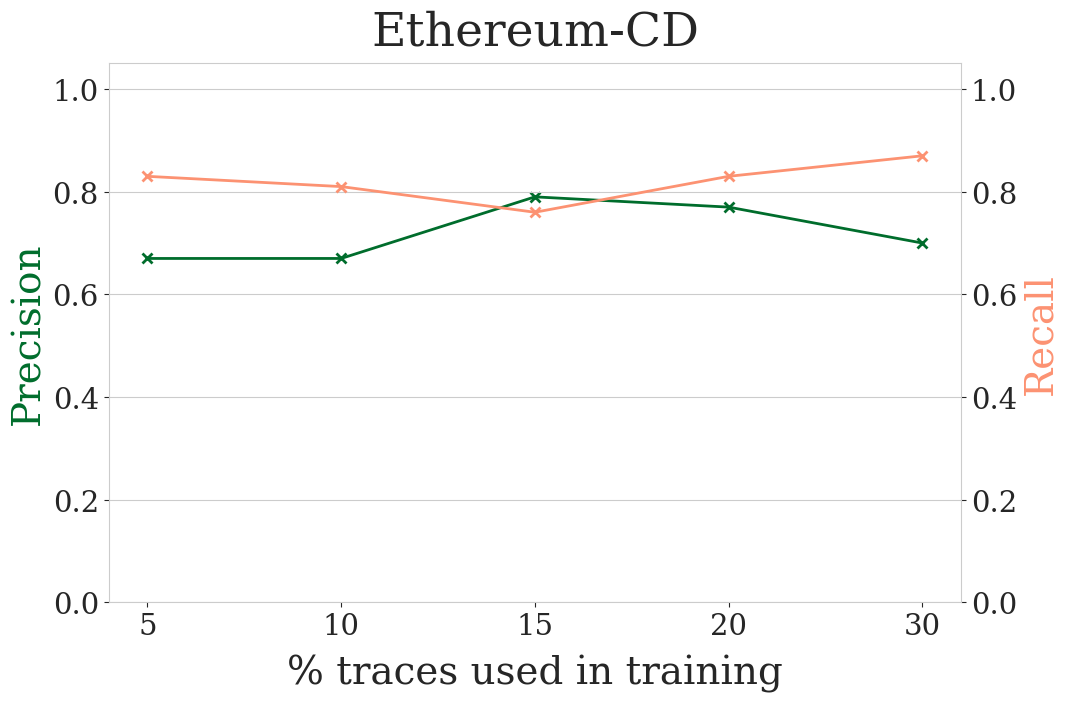
\includegraphics[scale=0.18]{6_9_eth_prec_rec_cd19_1.png}
        &
        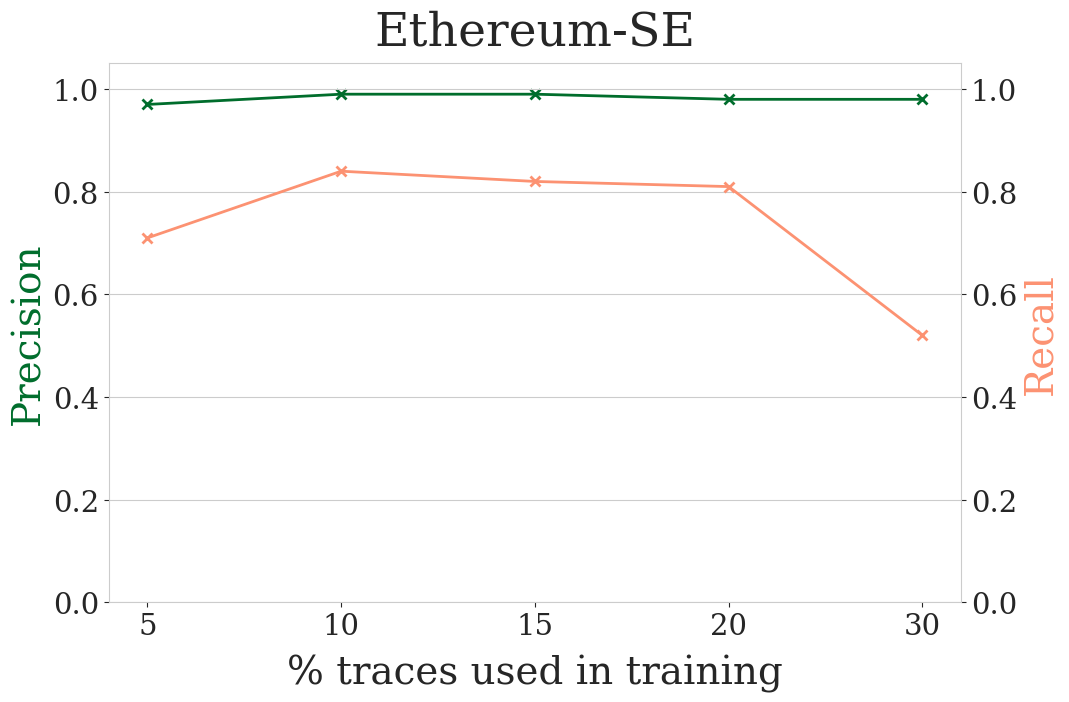
\includegraphics[scale=0.18]{6_9_eth_prec_rec_se13_1.png}
        &
        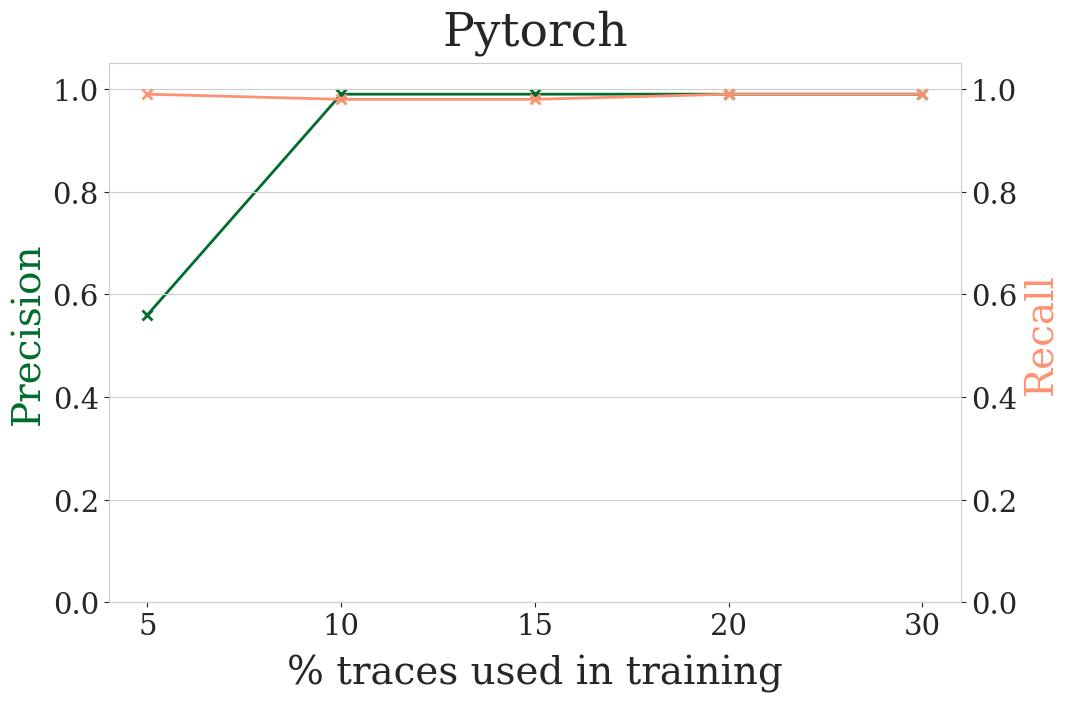
\includegraphics[scale=0.18]{6_26_pytorch_prec_rec.png}
        \\ [0.1cm]
		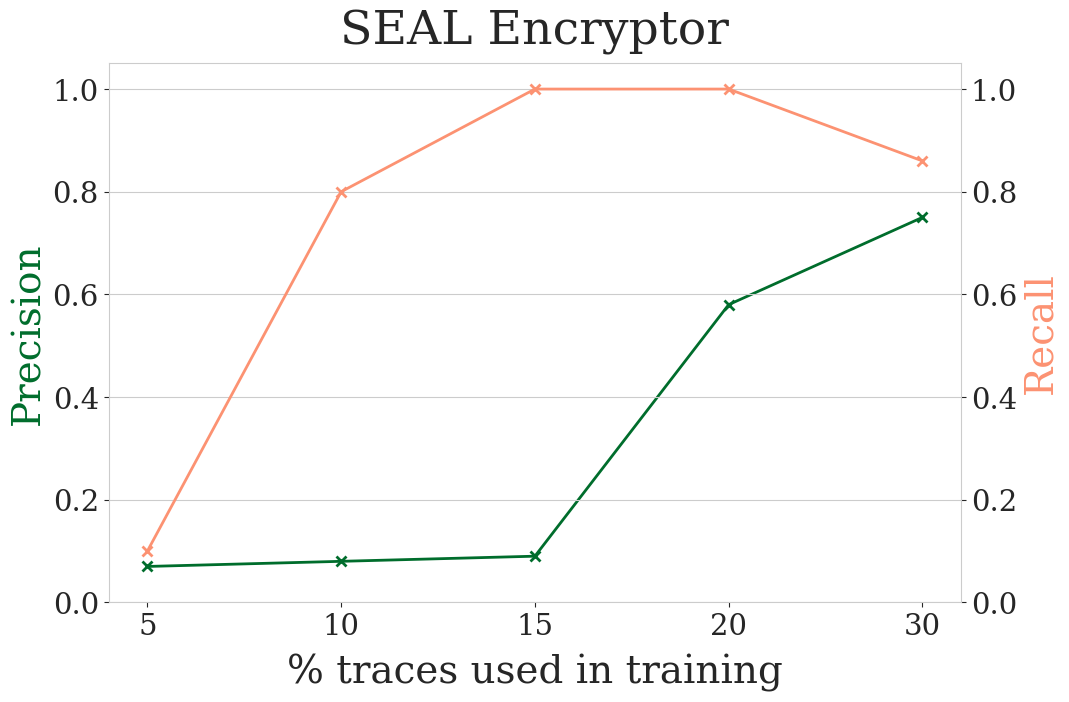
\includegraphics[scale=0.18]{6_1_sealencryptor_prec_rec.png}
		&
		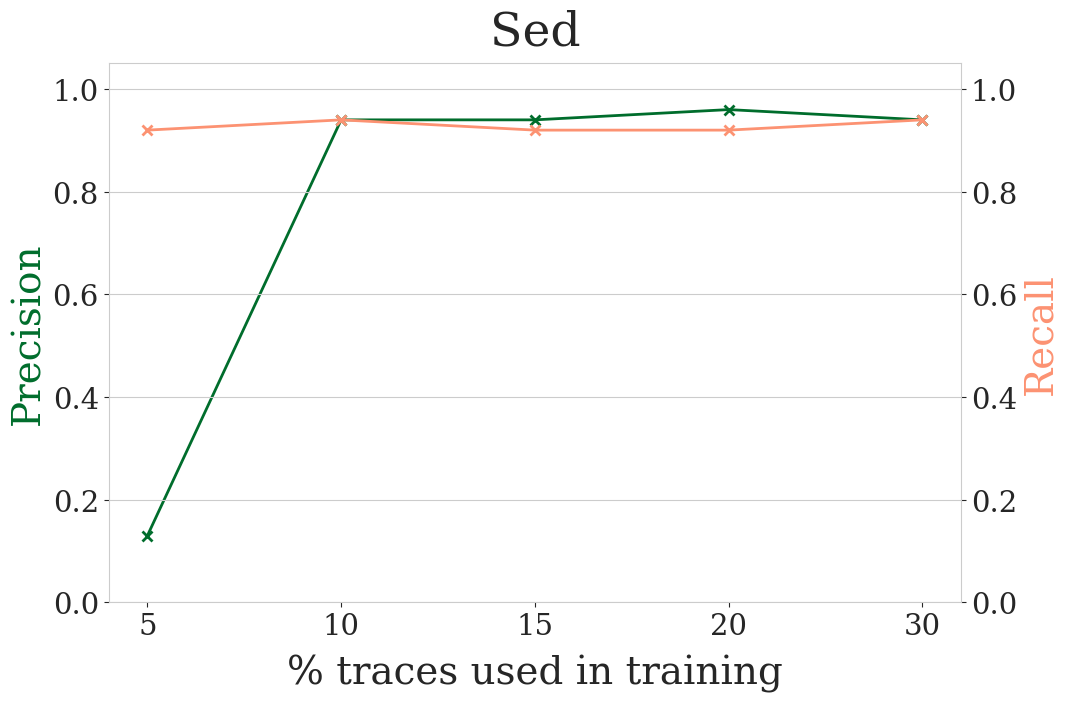
\includegraphics[scale=0.18]{6_24_sed_pr_rec.png}
%		&
%		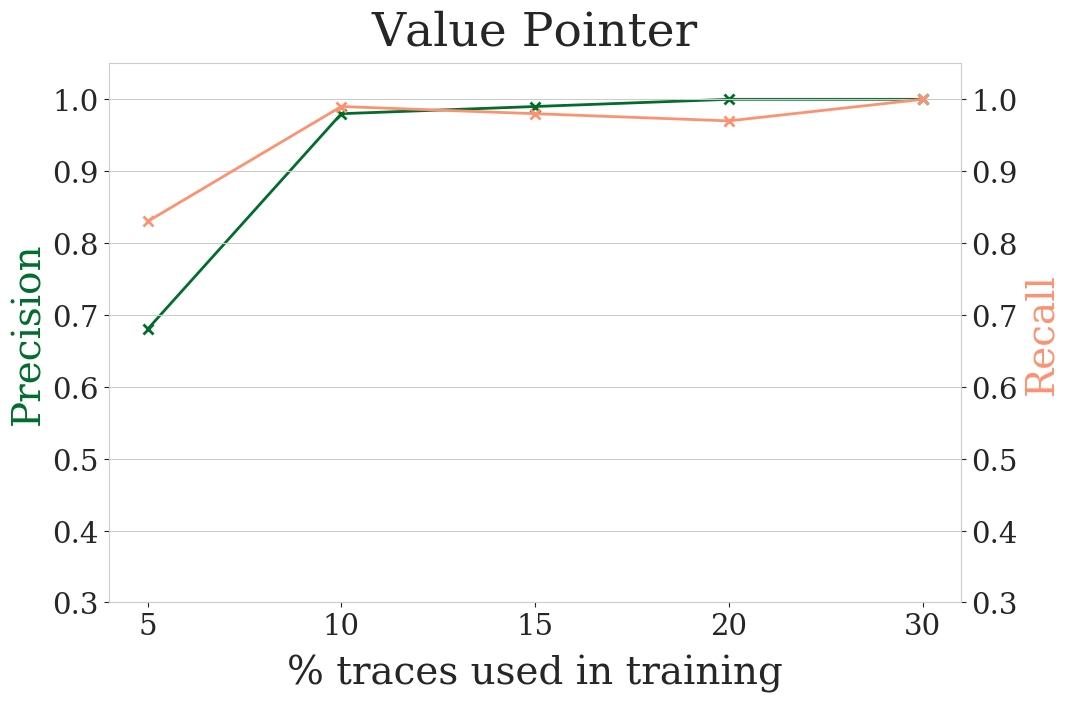
\includegraphics[scale=0.2]{6_25_valueptr_pr_rec.png}
		\\[0.1cm]
%		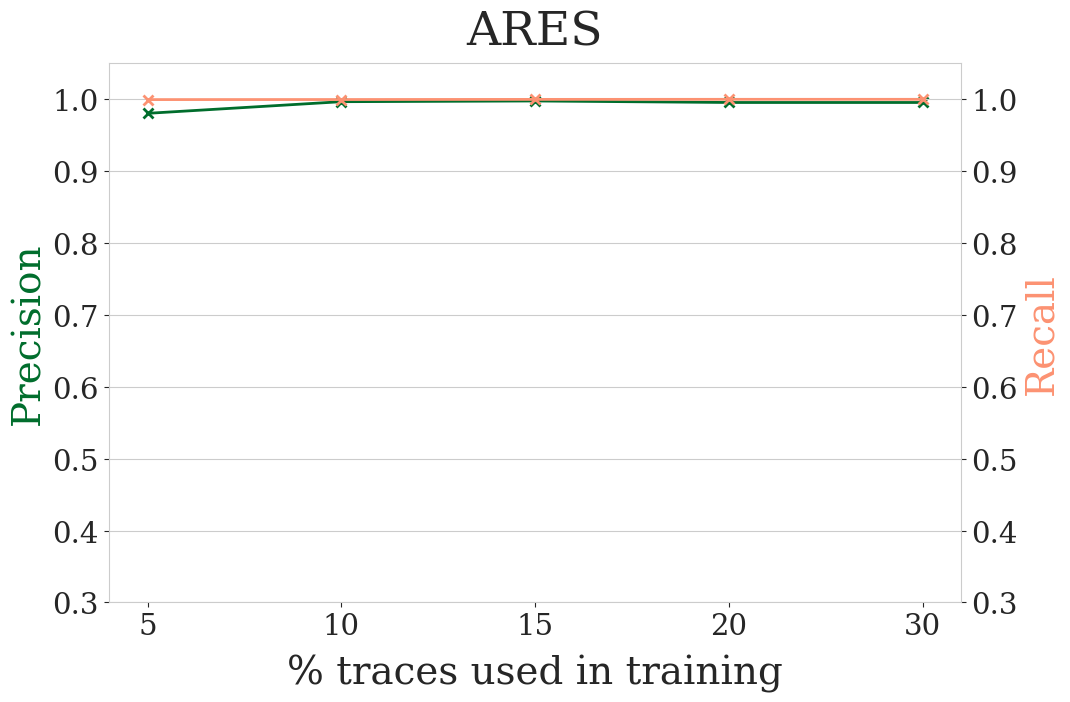
\includegraphics[scale=0.2]{6_16_fsmares_prec_rec.png}
%		&
%		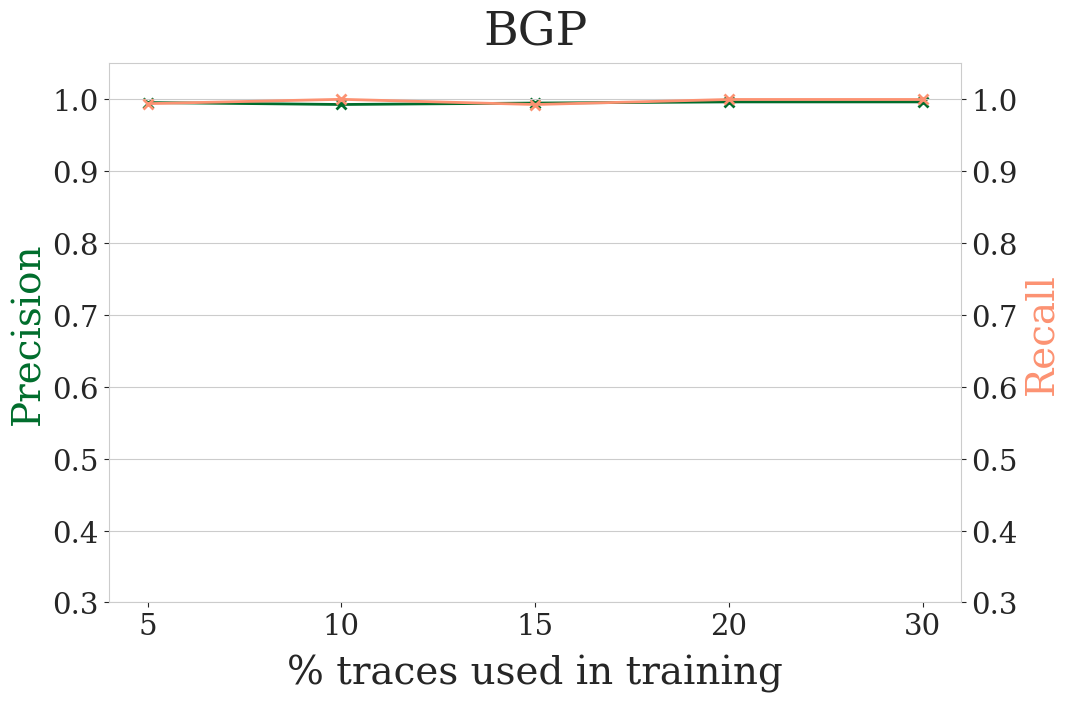
\includegraphics[scale=0.2]{6_15_fsmbgp_prec_rec.png}
%		&
%        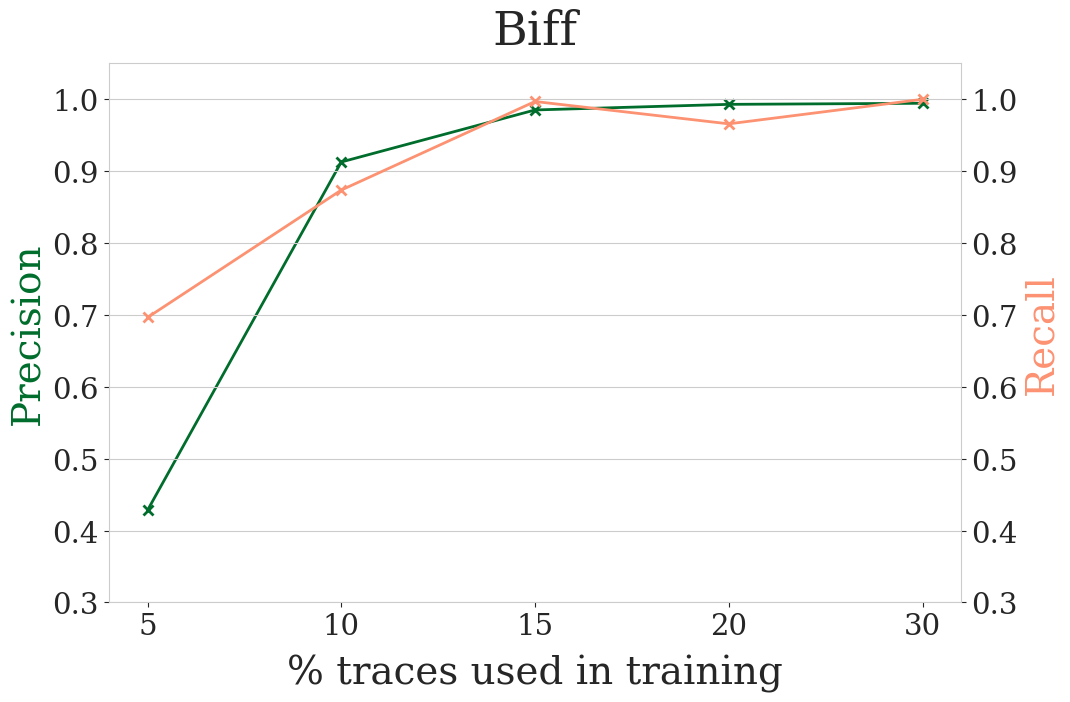
\includegraphics[scale=0.2]{6_3_fsmbiff_prec_rec.png}
%        \\[0.2cm]
%        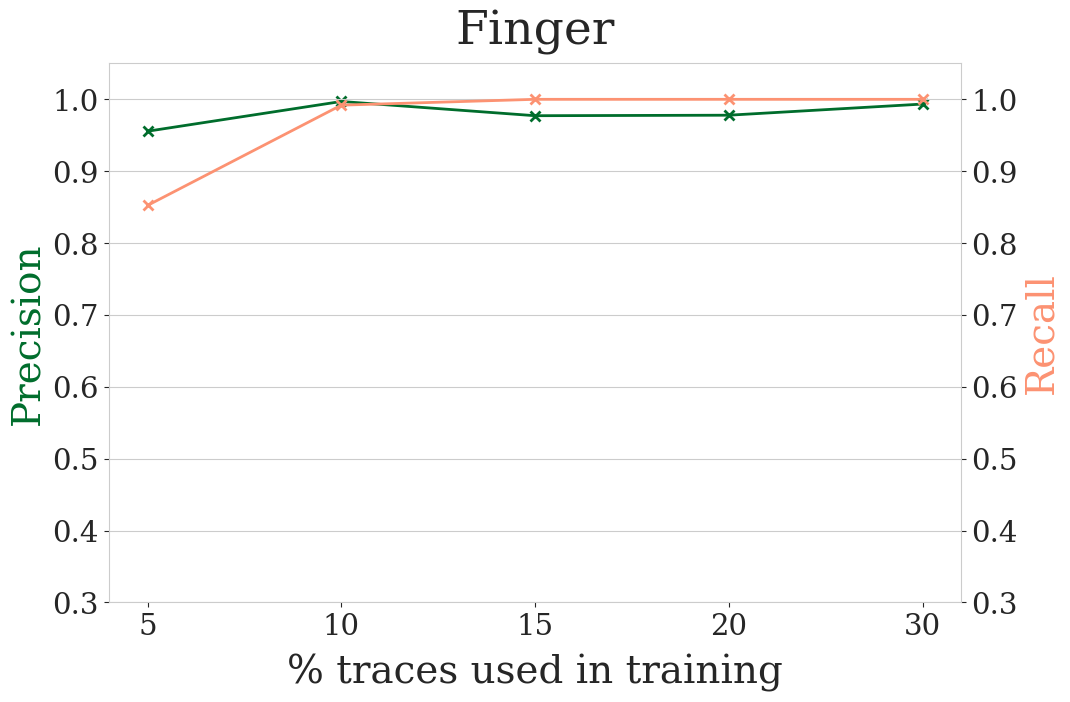
\includegraphics[scale=0.2]{6_14_fsmfinger_prec_rec.png}
%        &
%        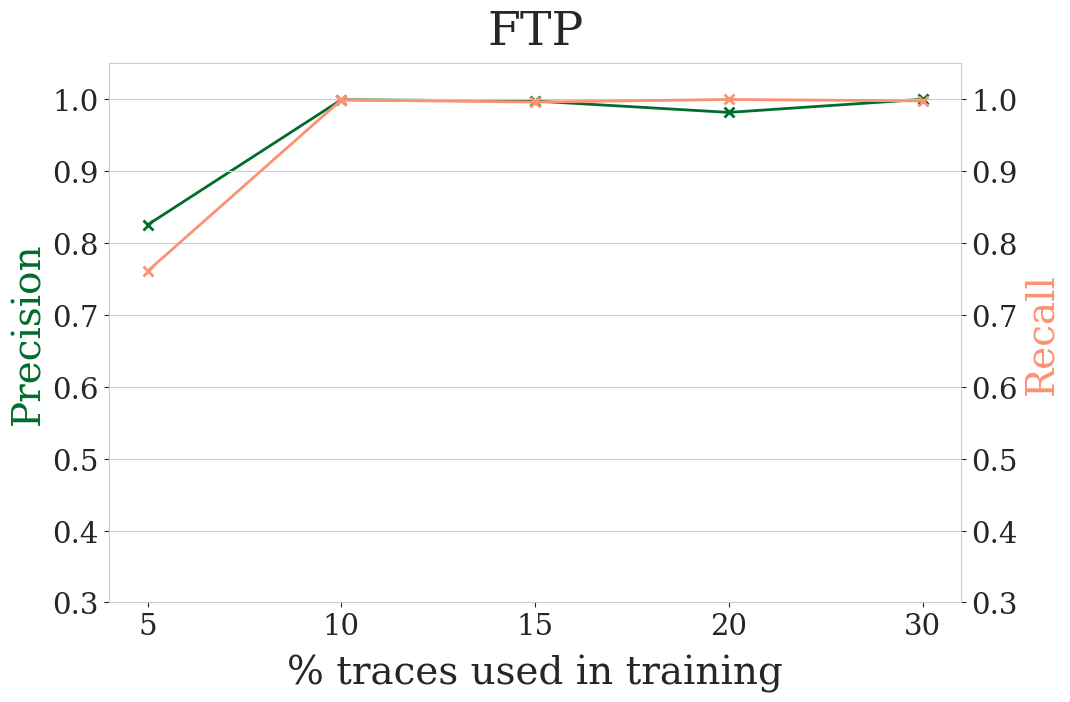
\includegraphics[scale=0.2]{6_13_fsmftp_prec_rec.png}
%        &
%        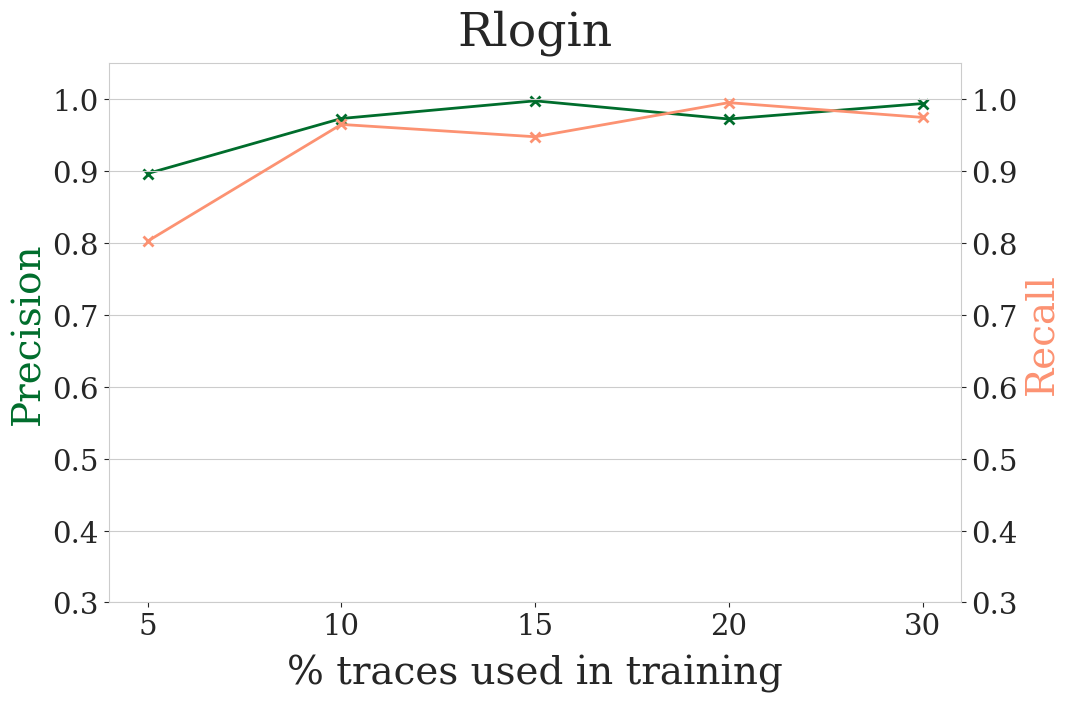
\includegraphics[scale=0.2]{6_12_fsmrlogin_prec_rec.png}
%        \\[0.2cm]
%        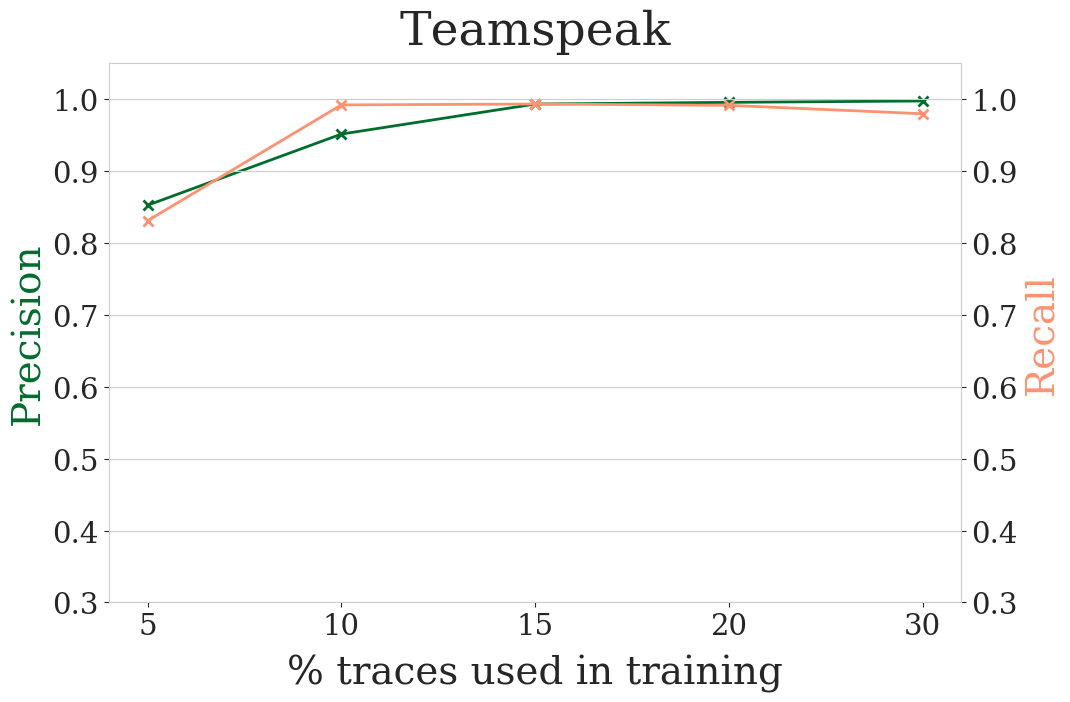
\includegraphics[scale=0.2]{6_10_fsmteamspeak_prec_rec.png}
%        &
% %       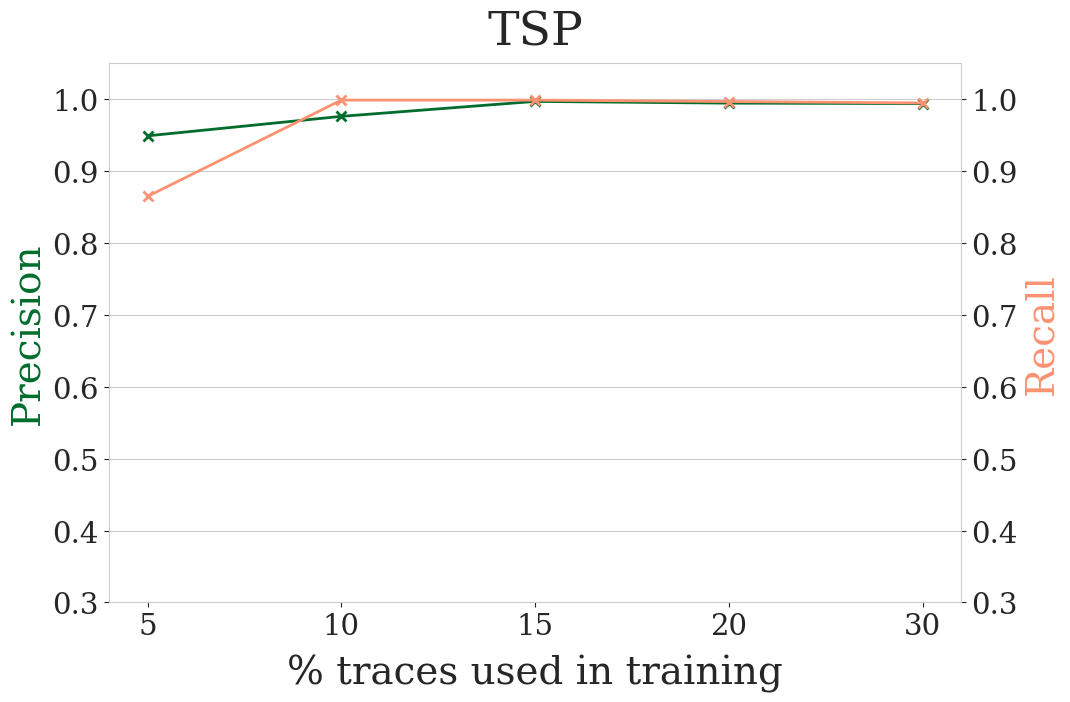
\includegraphics[scale=0.2]{6_17_fsmtsp_prec_rec.png}
% %       &
%        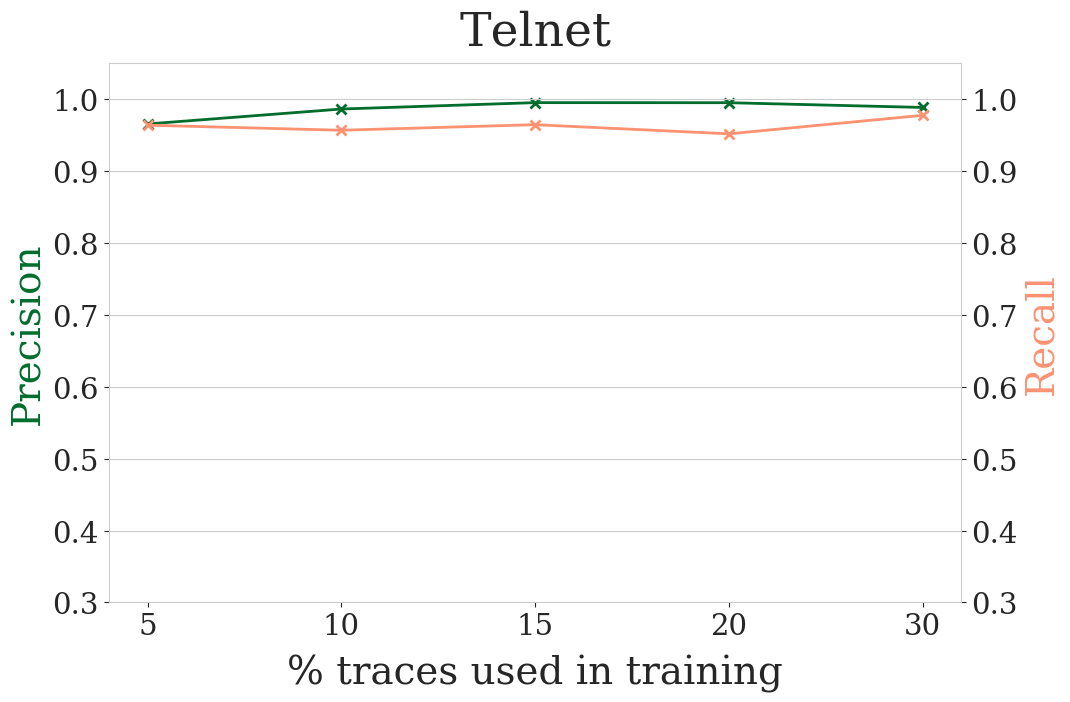
\includegraphics[scale=0.2]{6_11_fsmtelnet_prec_rec.png}
%        &
%        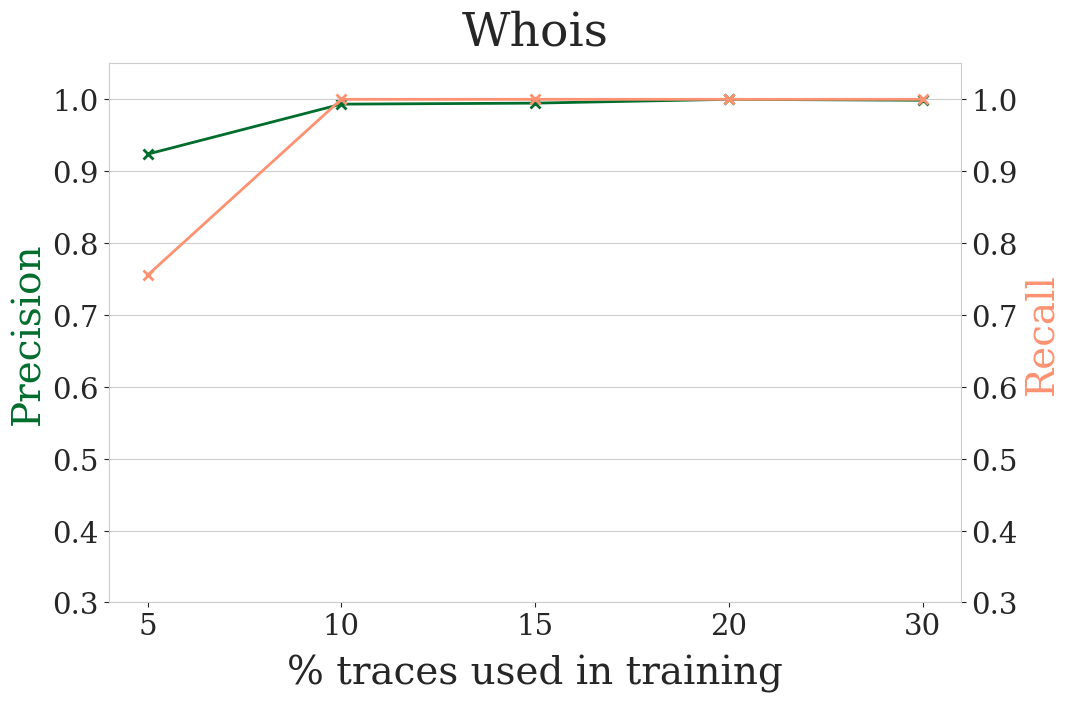
\includegraphics[scale=0.2]{6_4_fsmwhois_prec_rec.png}
%        \\ [0.2cm]
	\end{tabular}  
	\vspace{-10pt}
	\caption{Precision and recall achieved by classification model over each PUT.}
	\vspace{-5pt}
	\label{fig:precision-recall}
%	\Description[Precision and recall achieved by classification model over each PUT.]{}

\end{figure*}

%Figure~\ref{fig:precision-recall} shows fraction of traces used in training and its effect on precision and recall achieved by the classification model. 


Figure~\ref{fig:precision-recall} shows precision and recall achieved by our approach with different training set sizes.
The fraction of traces needed in training to achieve near maximal performance was 10\% to 30\% across the PUTs.
Excluding SEAL Encryptor, all the other programs only needed to be trained over 15\% of the traces to achieve near maximal performance. SEAL encryptor had very few failing traces, requiring a larger fraction of traces to get sufficient representation of failing classes during training. 
As seen in the plots in Figure~\ref{fig:precision-recall}, increasing the \% of traces used in training does not increase precision and recall for all PUTs. For instance, Pytorch and Sed observe a dramatic increase in precision and recall  when going from 5 to 10\% traces in training. Performance, however, stagnates after that point with increasing traces. With Ethereum-CD and Ethereum-SE, precision or recall becomes worse after 20\% traces. This maybe because the model is overfitting to the training traces.  
%Initially, increasing the size of training set results in better precision and recall. The extent of improvement depends on the program and execution traces. For instance, when training set size is increased from 5\% to 10\% of the overall traces, precision for \texttt{Encryptor} improves from 67\% to 95\%, while precision for \texttt{Biguint} increased steeply from 37\% to 95\%. Nevertheless, we find this observation to be true with diminishing results: after a certain point, increasing the training set size does not result in a noticeable improvement in precision and recall. We find this threshold, typically, to be between 10 to 15\%, across our subject programs.} %For the \texttt{Encryptor}, after achieving high precision with 10\% and 15\%of the traces, it drops slightly at 20\% and then goes back up to the high value at 40\%. This abnormality can occur when the model overfits to the passing traces in the training data \miltos{Is there a better way to explain this?}.  
%an average training set size of 492 traces,

It is also worth noting that the absolute size of our training set varies across subject programs. We find our approach works with training sets with as few as 3 failing traces to as many as 214. The range of passing tests in training was between 31 and 169.
\subsection{Q3. Comparison against state of art}
\label{sec:q3}

Table~\ref{tab:results} presents precision, recall, and specificity (TNR) achieved by the agglomerative hierarchical clustering proposed by Almaghairbe et al.~\cite{almaghairbe2017separating} on each of the PUTs. Comparing the precision, recall and TNR of our approach versus hierarchical clustering, we find our approach clearly outperforms the clustering approach on all but the Ethereum-CD PUT. This is because the hierarchical clustering assumption does not hold for these programs. According to this assumption, passing traces tend to be grouped in a few big clusters and failing traces are grouped into many small clusters. However, for these programs, passing traces tend to be grouped in many small clusters based on their call sequence pattern, making it hard to distinguish them from failing traces by simply comparing cluster sizes. 


With Ethereum-CD, the hierarchical clustering approach achieves precision and specificity of 100\% and a recall of 49\%. This is achieved with complete-linkage clustering, Euclidean distance and a cluster count equal to 10\% of total traces. In contrast our approach achieves a precision of 80\%, recall of 82\% and specificity of 79\%. To enable better comparison, we plot the precision-recall curve of the NN model in Figure~\ref{fig:roc} for Ethereum-CD, using 15\% of the traces in training. %\ajitha{Explain the precision recall curve and where the hierarchical clustering method falls.} %For certain programs, like the \texttt{Seal Encryptor}, the clustering approach achieves a slightly better recall ($1.0$ vs $0.98$) than our approach but the precision (of $0.5$) and TNR (of $0$) achieved with clustering are disappointing, making it unusable as it incorrectly classifies many failing and passing traces.  %The precision of $0.5$ and TNR of $0$ is, however, significantly lower than the $0.95$ precision and TNR achieved with our approach. This implies that the clustering approach does not incorrectly classify passing traces as failing, but does incorrectly classify failing traces as passing. 
%Figure~\ref{fig:roc} shows the precision and recall curve of \texttt{Ethereum-CD} when using 15\% of the traces for training. 

This curve shows the precision and recall of our trained model with respect to different values of the classification threshold.  It is clear from the plot that for the same value of recall (49\%), hierarchical clutering performs marginally better than our approach - 100\% versus 99\%. Hierarchical clustering works well over the Ethereum-CD PUT because the traces are clustered into just one big passing cluster and one failing cluster. Lack of cluster fragmentation improved accuracy of the hierarchical clustering approach. Nevertheless, our model achieves comparable performance for such traces. In addition, our model allows trade off between precision and recall by changing the classification threshold which may be driven by requirements or priorities of the use case. This tradeoff is not possible with the clustering approach. 


\begin{figure}[ht!]
\vspace{-8pt}
\centering
\includegraphics[scale=0.24]{../../figures/eth_roc_curve.png}
\vspace{-8pt}
\caption{Precision-Recall curve for \texttt{Ethereum-CD}.}
%\vspace{-20pt}
\label{fig:roc}
\vspace{-5pt}
\end{figure}
\iffalse
Overall, for 4 of the 5 subject programs, we find the clustering approach is unable to accurately distinguish failing and passing executions. This is because the hierarchical clustering assumption does not hold for these programs. According to this assumption, passing traces tend to be grouped in a few big clusters and failing traces are grouped into many small clusters. However, we find for 4 of our subject programs, passing traces also tend to be in many small clusters based on their call sequence pattern, making it hard to distinguish them from failing traces by simply comparing cluster sizes. 
However, for the Ethereum-CD program that the hierarchical clustering performs well over, the passing traces are grouped into one big cluster and the failing traces into another one. Size of the cluster of failing traces is smaller than the passing ones (despite a perfectly balanced dataset) as the technique incorrectly clusters some of the failing traces. 
\fi
%are grouped in large clusters for some programs as they have similar function call sequences as passing traces. This leads them to be incorrectly classified as passing in some cases. In addition, passing traces may also be grouped  into many small clusters when they have significant differences in method invocation sequences, especially for programs with heavy control flow, causing them to be incorrectly classified as failing in some instances. %Given the above, we also conclude that arguments and return values are vital information, therefore taking into account only callee name sequences significantly hinders classification accuracy.

%as the our approach has significantly higher accuracy than the clustering approach in correctly identifying and classifying both failing and passing traces. 
%Discuss each program and outliers. Average difference?

\iffalse
\textcolor{red}{\subsection{Q4. Generalisation}
\label{sec:q4}
In this research question, we conduct an initial exploration into the ambitious possibility of using a model, trained using traces from one subject program, to classify traces from other programs in the same application domain. We use FSMs from the network protocol domain to evaluate this possibility. Figures~\ref{biff_cross} and~\ref{whois_cross} represent precision and recall achieved by models trained using traces from \texttt{Biff} protocol and \texttt{Whois} protocol, respectively, to classify traces produced by other FSMs.
We find that the model trained using traces from \texttt{Biff} achieves high accuracy over the \texttt{Ares} protocol with precision and recall close to 1.0, and reasonable
precision ($ > 0.8$) for \texttt{BGP, FTP, Rlogin, Teamspeak, Whois} protocols. Lowest precision ($0.17$) was observed with \texttt{Telnet}. Average precision achieved in classifying traces from unseen FSMs was $0.79$.
Recall achieved by the model is lower than precision indicating that the model missed identifying failing traces in each of these protocols.  
Overall, the model trained with \texttt{Biff} traces was successful in identifying failing traces in other FSMs that have similar patterns to \texttt{Biff}. Failing traces with differing patterns were missed.  
We confirmed this observation by checking results from the \texttt{Whois} model. Although precision and recall numbers are different from the \texttt{Biff} model, the reasoning for classification success was the same - extent of similarity in execution patterns between FSMs.
%Although precision is higher, in general, than the average precision of the \texttt{Biff} model, the reasoning for higher recall was the same - extent of similarity in execution patterns between FSMs.
With the current approach, we find there is scope to generalise a classification model from a single FSM to multiple FSMs in the networking domain. However, achieving high accuracies with generalisation is a difficult problem and we plan to take small, definitive steps towards addressing this challenge in the future. As a next step, we will explore tuning the classification model from an individual FSM with sample traces from other FSMs to improve generalisation performance.  %and we believe that fine tuning or techniques like transfer learning will help 
}


\begin{figure}[ht!]
\centering
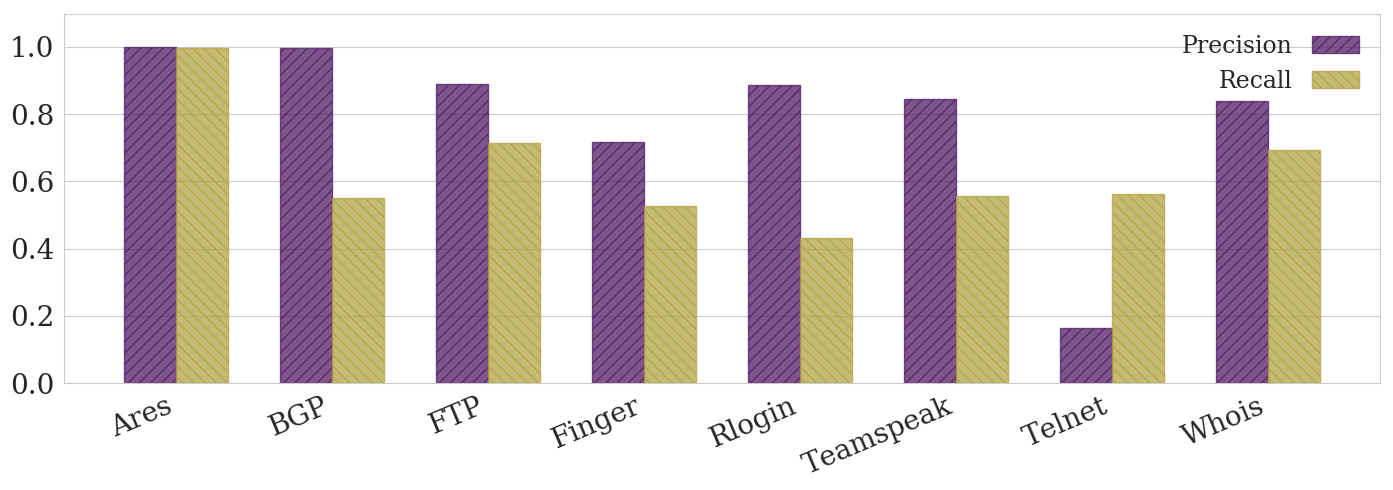
\includegraphics[scale=0.25]{6_5_biff_cross.png}
\vspace{-10pt}
\caption{\texttt{Biff} trained model - Precision and recall for unseen fsms.}
\Description[\texttt{Biff} trained model - Precision and recall for unseen fsms.]{}
\vspace{-10pt}
\label{biff_cross}
\end{figure}

\begin{figure}[ht!]
\centering
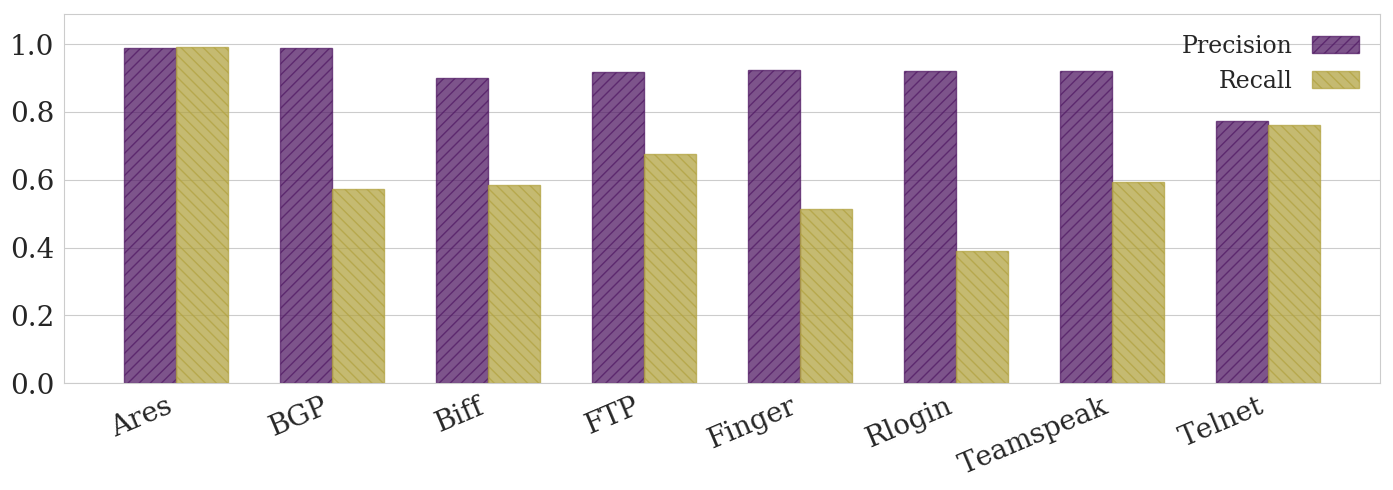
\includegraphics[scale=0.25]{6_6_whois_cross.png}
\vspace{-10pt}
\caption{\texttt{Whois} trained model - Precision and recall for unseen fsms.}
\Description[\texttt{Whois} trained model - Precision and recall for unseen fsms.]{}
\vspace{-15pt}
\label{whois_cross}
\end{figure}
\fi
\subsection{Threats to Validity}
\label{sec:threats}
We see three threats to validity of our
experiment based on the selection of subject programs and associated tests. 

%The subject programs in our experiment, expected output is provided with the tests and that is used for labelling the traces. 
%If the tests fo not specify the expected outputs, then a developer or expert would have to manually label the traces used in training, which is 
%a small fraction of the total traces that they would otherwise have to label. 
First, PUTs for 3 out of the 4 subject programs in our experiment were generated by seeding faults into a reference implementation. A reference implementation with only passing tests is not suitable for evaluating our approach.  To address this, we generated a faulty implementation and ran the original tests through the PUT to gather both passing and failing traces.  
%To avoid an imbalanced training set, we generated failing execution traces using seeded faults representing common bug patterns~\cite{jia2011analysis, pradel2018deepbugs}. %mutating passing test inputs and checking if they cause the actual output to differ from the expected output. 
It is possible using real faults in place of seeded faults may lead to
different results. However, Andrews et al. have shown the use of seeded faults leads to conclusions
similar to those obtained using real faults~\cite{andrews2006using, Do1707670}. 
For one of the subject programs, Sed,  we did not artificially seed faults, but instead used the existing implementation as it was accompanied by both passing and failing tests. % which helps mitigate this threat. 

Second, the number of tests that accompanied our subject programs was not very large, ranging from 132 to 2254 tests. The NN models in our experiments produced good performance with small to medium sized test suites that may be automatically or manually generated. Our approach is constrained by the amount of training data and not by the size of the test suite. As a result for programs accompanied by large test suites, the NN model will need a larger training set (fraction of traces to be used in training might still be 15\%). Nevertheless, the labelling effort for a fraction of the tests in our approach is still less than the current practise of labelling all the tests. 
%Although our experiment lacks subject programs with a large test suite, we believe achieving good performance over approach is well suited to NN models for programs with larger test sets will perform  
%These programs did not have adequate tests that can be used for training and evaluation. 

%This was done to increase the size of data set available training and evaluation. 

Finally, we conducted our study on subject programs from 4 different application domains which is not representative of all application domains. %The NN model in our approach is learned and trained for each subject program and used to classify traces for just that program. 
Given that our approach has no domain specific constraints, we believe it will be widely applicable. %owill result in high accuracy test classification for subject programs in other domains as well. 
%We believe our approach for learnign a model to classify traces will work well for programs in other domains as well as there is no 
%We believe these systems are representative of the class of systems in which we are interested, and our
%results are thus generalizable to other systems in the domain.


\iffalse
Another threat to external validity relates
to the test suites used in our study. 
We used existing test suites for the SIR programs and randomly generated test suites that are controlled for 
test suite size for the EEMBC programs and LLVM Symbolizer. 
We cannot claim that the test
suites we used are necessarily representative of all possible
test suites.
Additional
research is needed to assess the performance of locality ordering with
different test generation frameworks
and with hand-written tests.
\fi

\iffalse

\begin{table}[]
\centering
%\iffalse
\begin{tabular}{|c|c|c|c|c|}
	\hline
	Trace section omitted   & {Precision} & {Recall} & TNR\\ 
	\hline \hline
	Function names  & 0.49 & 0.98 & 0.02 \\ \hline 
	Return values & 0.50  & 0.94 & 0.07 \\ \hline
	Arguments & 0.52  & 0.91 & 0.36 \\ \hline
	Half the \#trace lines & 0.70 & 0.86 & 0.63 \\ \hline 
\end{tabular}
%\fi
\caption{Precision and Recall of models trained with traces omitting certain information for \texttt{Ethereum}. }
\label{tab:ethereum_removed_trace}
\end{table}

\begin{table}[]
\centering
%\iffalse
\begin{tabular}{|c|c|c|c|c|}
	\hline
	Trace section omitted   & {Precision} & {Recall} & TNR\\ 
	\hline \hline
	Function names  & 0.92 & 0.14 & 0.98 \\ \hline 
	Return values & 0.79  & 0.98 & 0.74 \\ \hline
	Arguments & 0.70  & 0.98 & 0.59 \\ \hline
	Half the \#trace lines & 0.72 & 1.0 & 0.58 \\ \hline 
\end{tabular}
%\fi
\caption{Precision and Recall of models trained with traces omitting certain information for \texttt{Encryptor}. }
\label{tab:encryptor_removed_trace}
\end{table}

\begin{table}[]
\centering
%\iffalse
\begin{tabular}{|c|c|c|c|c|}
	\hline
	Trace section omitted   & {Precision} & {Recall} & TNR\\ 
	\hline \hline
	Function names  & 0.95 & 0.58 & 0.97 \\ \hline 
	Return values & 0.97  & 0.94 & 0.97 \\ \hline
	Arguments & 0.90  & 0.88 & 0.91 \\ \hline
	Half the \#trace lines & 0.81 & 0.90 & 0.79 \\ \hline 
\end{tabular}
%\fi
\caption{Precision and Recall of models trained with traces omitting certain information for \texttt{Biguint}. }
\label{tab:biguint_removed_trace}
\end{table}

\begin{table}[]
\centering
%\iffalse
\begin{tabular}{|c|c|c|c|c|}
	\hline
	Trace section omitted   & {Precision} & {Recall} & TNR\\ 
	\hline \hline
	Function names  & 0.62 & 0.86 & 0.37 \\ \hline 
	Return values & 0.47  & 1.0 & 0.0 \\ \hline
	Arguments & 0.52  & 0.96 & 0.04 \\ \hline
	Half the \#trace lines & 0.47 & 1.0 & 0.0 \\ \hline 
\end{tabular}
%\fi
\caption{Precision and Recall of models trained with traces omitting certain information for \texttt{Value pointer}. }
\label{tab:valueptr_removed_trace}
\end{table}



\begin{table}[]
\centering
%\iffalse
\begin{tabular}{|c|c|c|c|c|}
	\hline
	Trace section omitted   & {Precision} & {Recall} & TNR\\ 
	\hline \hline
	Function names  & 0.11 & 1.0 & 0.02 \\ \hline 
	Return values & 0.20  & 0.24 & 0.89 \\ \hline
	Arguments & 0.67  & 0.08 & 0.99 \\ \hline
	Half the \#trace lines & 1.0 & 0.08 & 1.0 \\ \hline 
\end{tabular}
%\fi
\caption{Precision and Recall of models trained with traces omitting certain information for \texttt{Sed}. }
\label{tab:sed_removed_trace}
\end{table}


\begin{table}[]
\centering
%\iffalse
\begin{tabular}{|c|c|c|c|c|}
	\hline
	Trace section omitted   & {Precision} & {Recall} & TNR\\ 
	\hline \hline
	Function names  & 0.96 & 0.98 & 0.95 \\ \hline 
	Return values & 0.95  & 0.99 & 0.75 \\ \hline
	Arguments & 0.93  & 0.96 & 0.68 \\ \hline
	Half the \#trace lines & 0.99 & 0.99 & 0.79 \\ \hline
	Global state & 0.95 & 0.96 & 0.97 \\ \hline 
\end{tabular}
%\fi
\caption{Precision and Recall of models trained with traces omitting certain information for \texttt{Ares} protocol. }
\label{tab:ares_removed_trace}
\end{table}


\begin{table}[]
\centering
%\iffalse
\begin{tabular}{|c|c|c|c|c|}
	\hline
	Trace section omitted   & {Precision} & {Recall} & TNR\\ 
	\hline \hline
	Function names  & 0.99 & 0.98 & 0.98 \\ \hline 
	Return values & 0.98 & 0.99 & 0.98 \\ \hline
	Arguments & 0.97  & 0.97 & 0.97 \\ \hline
	Half the \#trace lines & 0.62 & 0.84 & 0.48 \\ \hline
	Global state & 0.62 & 0.87 & 0.47 \\ \hline
\end{tabular}
%\fi
\caption{Precision and Recall of models trained with traces omitting certain information for \texttt{BGP} protocol. }
\label{tab:bgp_removed_trace}
\end{table}



\begin{table}[]
\centering
%\iffalse
\begin{tabular}{|c|c|c|c|c|}
	\hline
	Trace section omitted   & {Precision} & {Recall} & TNR\\ 
	\hline \hline
	Function names  & 0.58 & 0.84 & 0.41 \\ \hline 
	Return values & 0.56 & 0.92 & 0.35 \\ \hline
	Arguments & 0.51  & 0.64 & 0.40 \\ \hline
	Half the \#trace lines & 0.51 & 0.81 & 0.23 \\ \hline
	Global state & 0.62 & 0.76 & 0.55 \\ \hline
\end{tabular}
%\fi
\caption{Precision and Recall of models trained with traces omitting certain information for \texttt{Biff} protocol. }
\label{tab:biff_removed_trace}
\end{table}


\begin{table}[]
\centering
%\iffalse
\begin{tabular}{|c|c|c|c|c|}
	\hline
	Trace section omitted   & {Precision} & {Recall} & TNR\\ 
	\hline \hline
	Function names  & 0.99 & 0.95 & 0.99 \\ \hline 
	Return values & 0.98 & 0.97 & 0.99 \\ \hline
	Arguments & 0.52  & 0.19 & 0.88 \\ \hline
	Half the \#trace lines & 0.49 & 0.60 & 0.59 \\ \hline
	Global state & 0.97 & 0.94 & 0.97 \\ \hline
\end{tabular}
%\fi
\caption{Precision and Recall of models trained with traces omitting certain information for \texttt{Finger} protocol. }
\label{tab:finger_removed_trace}
\end{table}


\begin{table}[]
\centering
%\iffalse
\begin{tabular}{|c|c|c|c|c|}
	\hline
	Trace section omitted   & {Precision} & {Recall} & TNR\\ 
	\hline \hline
	Function names  & 0.99 & 0.99 & 0.98 \\ \hline 
	Return values & 0.97 & 0.97 & 0.98 \\ \hline
	Arguments & 0.88  & 0.93 & 0.84 \\ \hline
	Half the \#trace lines & 0.71 & 0.91 & 0.52 \\ \hline
	Global state & 0.96 & 0.96 & 0.98 \\ \hline 
\end{tabular}
%\fi
\caption{Precision and Recall of models trained with traces omitting certain information for \texttt{FTP} protocol. }
\label{tab:ftp_removed_trace}
\end{table}

\begin{table}[]
\centering
%\iffalse
\begin{tabular}{|c|c|c|c|c|}
	\hline
	Trace section omitted   & {Precision} & {Recall} & TNR\\ 
	\hline \hline
	Function names  & 0.95 & 0.96 & 0.96 \\ \hline 
	Return values & 1.0 & 0.92 & 1.0 \\ \hline
	Arguments & 0.85  & 0.91 & 0.94 \\ \hline
	Half the \#trace lines & 0.93 & 0.93 & 0.97 \\ \hline
	Global state & 0.92 & 0.95 & 0.92 \\ \hline 
\end{tabular}
%\fi
\caption{Precision and Recall of models trained with traces omitting certain information for \texttt{Rlogin} protocol. }
\label{tab:rlogin_removed_trace}
\end{table}

\begin{table}[]
\centering
%\iffalse
\begin{tabular}{|c|c|c|c|c|}
	\hline
	Trace section omitted   & {Precision} & {Recall} & TNR\\ 
	\hline \hline
	Function names  & 0.91 & 0.97 & 0.91 \\ \hline 
	Return values & 0.94 & 0.98 & 0.94 \\ \hline
	Arguments & 0.77  & 0.86 & 0.77 \\ \hline
	Half the \#trace lines & 0.93 & 0.93 & 0.97 \\ \hline
	Global state & 0.90 & 0.93 & 0.91 \\ \hline 
\end{tabular}
%\fi
\caption{Precision and Recall of models trained with traces omitting certain information for \texttt{Teamspeak} protocol. }
\label{tab:teamspeak_removed_trace}
\end{table}


\begin{table}[]
\centering
%\iffalse
\begin{tabular}{|c|c|c|c|c|}
	\hline
	Trace section omitted   & {Precision} & {Recall} & TNR\\ 
	\hline \hline
	Function names  & 0.88 & 1.0 & 0.49 \\ \hline 
	Return values & 0.82 & 1.0 & 0.25 \\ \hline
	Arguments & 0.76  & 1.0 & 0.0 \\ \hline
	Half the \#trace lines & 0.75 & 0.93 & 0.0 \\ \hline
	Global state & 0.88 & 1.0 & 0.49 \\ \hline 
\end{tabular}
%\fi
\caption{Precision and Recall of models trained with traces omitting certain information for \texttt{Telnet} protocol. }
\label{tab:telnet_removed_trace}
\end{table}
%
\begin{table}[]
\centering
%\iffalse
\begin{tabular}{|c|c|c|c|c|}
	\hline
	Trace section omitted   & {Precision} & {Recall} & TNR\\ 
	\hline \hline
	Function names  & 0.96 & 0.97 & 0.96 \\ \hline 
	Return values & 0.94 & 0.97 & 0.96 \\ \hline
	Arguments & 0.94  & 0.97 & 0.96 \\ \hline
	Half the \#trace lines & 0.85 & 0.94 & 0.90 \\ \hline
	Global state & 0.93 & 0.95 & 0.92 \\ \hline 
\end{tabular}
%\fi
\caption{Precision and Recall of models trained with traces omitting certain information for \texttt{TSP} protocol. }
\label{tab:tsp_removed_trace}
\end{table}

\begin{table}[]
\centering
%\iffalse
\begin{tabular}{|c|c|c|c|c|}
	\hline
	Trace section omitted   & {Precision} & {Recall} & TNR\\ 
	\hline \hline
	Function names  & 0.96 & 0.96 & 0.96 \\ \hline 
	Return values & 0.96 & 0.96 & 0.96 \\ \hline
	Arguments & 0.72  & 0.75 & 0.73 \\ \hline
	Half the \#trace lines & 0.58 & 0.61 & 0.60 \\ \hline
	Global state & 0.96 & 0.96 & 0.96 \\ \hline 
\end{tabular}
%\fi
\caption{Precision and Recall of models trained with traces omitting certain information for \texttt{Whois} protocol. }
\label{tab:whois_removed_trace}
\end{table}

\fi

\iffalse
\begin{table*}[]
\centering
\small
\begin{tabular}{|l|l|l|l|l|l@{\hskip 5mm}|l|l|l|}
	\hline
	Mutation & CD1 & CD9 & CD10 & CD19 & CD20 \\ 
	\hline
	5\% & 0.65, 0.91, 0.51 & 0.99, 0.63, 0.99 & 0.86, 0.70, 0.88 & 0.67, 0.83, 0.59 & 0.64, 0.93, 0.50  \\ \hline
	10\% & 0.92, 0.70, 0.94 & 0.70, 0.94, 0.60 & 0.64, 0.81, 0.51 & 0.67, 0.81, 0.61 & 0.76, 0.84, 0.73 \\ \hline
	15\% & 0.78, 0.74, 0.80 & 0.74, 0.82, 0.74 & 0.84, 0.77, 0.86 & 0.79, 0.76, 0.79 & 0.76, 0.73, 0.77 \\ \hline
	20\% & 0.83, 0.80, 0.83 & 0.89, 0.72, 0.91 & 0.82, 0.67, 0.86 & 0.77, 0.83, 0.74 & 0.80, 0.80, 0.80 \\ \hline
	30\% & 0.86, 0.71, 0.88 & 0.91, 0.74, 0.92 & 0.77, 0.81, 0.76 & 0.70, 0.87, 0.64 & 0.75, 0.83, 0.72 \\
	\hline
\end{tabular}
\caption{Pr, Rec, TNR for each ethereum mutation with respect to the size of training set (\textcolor{red}{Ratio in these mutations: 1127 pass, 1127 fail})}
\vspace{-20pt}
\label{tab:eth-1}
\end{table*}



\begin{table*}[]
\centering
\small
\begin{tabular}{|l|l|l|l|l|l|l@{\hskip 5mm}|l|l|l|}
	\hline
	Mutation & SE13 (92p, 2162f) & SE16 (1334p, 920f) & SE17 (1334p, 920f) & SE18 (1426p, 828f) \\ 
	\hline
	5\% & 0.97, 0.71, 0.59 & 1, 1, 1 & 0.99, 0.99, 0.99 & 0.88, 0.97, 0.92 \\ \hline
	10\% & 0.99, 0.84, 0.73 & 1, 1, 1 & 0.97, 0.97, 0.98 & 0.90, 0.94, 0.94 \\ \hline
	15\% & 0.99, 0.82, 0.86 & 1, 1, 1 & 0.96, 0.96, 0.97 & 0.86, 0.97, 0.91 \\ \hline
	20\% & 0.98, 0.81, 0.58 & 1, 1, 1 & 0.92, 0.93, 0.94 & 0.89, 0.91, 0.94 \\ \hline
	30\% & 0.98, 0.52, 0.75 & 1, 1, 1 & 0.96, 0.97, 0.98 & 0.99, 0.99, 0.99 \\ \hline
\end{tabular}
\caption{Pr, Rec, TNR for each ethereum mutation with respect to the size of training set, with ratio embedded in title}
\vspace{-20pt}
\label{tab:eth-2}
\end{table*}


\begin{table*}[]
\centering
\small
\begin{tabular}{|l|l|l|l|l|l|l@{\hskip 5mm}|l|l|l|}
	\hline
	Mutation & Func names & Return val & Arguments & Half trace \\ 
	\hline
	5\% & 0.70, 0.72, 0.69 & 0.72, 0.73, 0.72 & 0.52, 0.82, 0.26 & 0.69, 0.85, 0.61 \\ \hline
	10\% & 0.74, 0.76, 0.74 & 0.71, 0.92, 0.64 & 0.59, 0.82, 0.44 & 0.82, 0.80, 0.83 \\ \hline
	15\% & 0.75, 0.85, 0.70 & 0.81, 0.72, 0.84 & 0.66, 0.83, 0.56 & 0.73, 0.77, 0.71 \\ \hline
	20\% & 0.94, 0.64, 0.97 & 0.50, 0.89, 0.11 & 0.79, 0.69, 0.82 & 0.94, 0.68, 0.96 \\ \hline
	30\% & 0.92, 0.66, 0.94 & 0.82, 0.81, 0.81 & 0.71, 0.92, 0.62 & 0.89, 0.70, 0.91 \\ \hline
\end{tabular}
\caption{Pr, Rec, TNR for CD1 mutation, ablation study}
\vspace{-20pt}
\label{tab:eth-3}
\end{table*}


\begin{table*}[]
\centering
\small
\begin{tabular}{|l|l|l|l|l|l|l@{\hskip 5mm}|l|l|l|}
	\hline
	Mutation & Func names & Return val & Arguments & Half trace \\ 
	\hline
	10\% & 0.63, 0.64, 0.62 & 0.68, 0.87, 0.60 & 0.54, 0.78, 0.35 & 0.81, 0.83, 0.80 \\ \hline
\end{tabular}
\caption{Pr, Rec, TNR for CD19 mutation, ablation study}
\vspace{-20pt}
\label{tab:eth-4}
\end{table*}

\fi

%%%%%%%%%%%%%%%%%%%%%%%%%55

\iffalse
\foivos{Below, I am writing all my comments and reasons related to the training results and the ablation study results.}

Encryptor:
\begin{itemize}
\item Set contains 11 failing and 122 passing tests
\item Using small training set means that you get at best 2 failing samples, therefore precision is expected to be low
\item 11 failing tests have exactly the same call sequence, because mutation broke a specific functionality, apparently invoked from this group.
\item There is variety between the passing ones.
\end{itemize}



Pytorch
\begin{itemize}
\item There is a large difference in their length between passing and failing traces. Failing traces are much smaller.
\item In practise, this means that the control flow of failing tests either ends earlier, or it is diverged to a different part of the codebase that we have not instrumented (Remember, we do not and absolutely cannot instrument all the codebase. We focus on 5-6 source files of interest).
\end{itemize}


Ethereum CD
\begin{itemize}
\item Mutation happens to function fromHexChar. This function takes a hex char and returns its decimal number (e.g. f('a') = 10).
\item Mutation happens in one of the three branches: if input char is between 'a' and 'f' it should return input-'a'+10.
\item Mutation turns + to *.
\item This function is not called from the core difficulty calculation function which is tested. It is only called from internal functions within the same source file. These internals are as well not called by any of libethcore files (the module where the  diff calc method belongs). That means that its impact is very deep in the control flow.
\item Makes half tests pass, half tests fail.
\end{itemize}

Ethereum CD ablation study:
\begin{itemize}
\item Removing lower part of trace improves metrics, which proves that critical information about this mutation is to be found in the early part of the trace. Maybe this is a chance to mention that localizing the bug is also important but difficult for now.
\end{itemize}

Ethereum SE
\begin{itemize}
\item Mutation happens in the core function of difficulty calculation.
\item Due to the mutation, instead of very large integers being subtracted to avoid overflow, the subtraction takes place on smaller ones.
\item When test inputs have the values that will lead to the mutated condition to exeute, the function will return the wrong output.
\item This wrong output is expected to be seen i) towards the very end of the trace, ii) In the return field of the mutated function and iii) to the argument section of intermediate functions called.
\end{itemize}

Sed
\begin{itemize}
\item Failing tests present a sequence of calls to a function called getChar, towards the end. Calls to this function does not appear in passing traces.
\item Length and format between failing and passing looks similar.
\item Failing traces are again few (18), at least 2 are needed as a sample.
\end{itemize}

Sed ablation study
\begin{itemize}
\item Removing the function names produces the worst results. This might mean that this call sequence found in failing traces is indeed the feature that distincts the two classes.
\end{itemize}

\fi


\vspace{-5pt}
\section{Conclusion}
\label{sec:future}
In this paper, we propose a novel approach for designing a test oracle as a NN model, learning from execution traces of a given program. 
We have implemented an end to end framework for automating the steps in our approach, (1) Gathering execution traces as sequences of method invocations, (2) Encoding variable length execution traces into a fixed length vector, (3) Designing a NN model that uses the trace information to classify the trace as pass or fail. 
%Our approach handles unbalanced test sets with unequal passing and failing traces by weighting the samples accordingly. 

We evaluated the approach using 5 realistic PUTs and tests. We found the classification model for each PUT was effective in classifying passing and failing executions, achieving an average of 89\% precision, 88\% recall and 92\% specificity while only training with an average 15\% of the total traces. %Most subject programs use approximately 10\% of the traces for training to achieve maximum performance. 
%For programs with a large number of traces, a lower proportion of traces was adequate for training. 
We outperform the hierarchical clustering technique proposed in recent literature by a large margin of accuracy for 4 out of the 5 PUTs, and achieved comparable performance for the other PUT.

\paragraph{Practical use} Our approach can be applied out of the box for classifying tests for any software that can be compiled to LLVM IR. We gather execution traces for test inputs automatically, and require a small fraction of the traces to be labelled with their pass or fail outcomes (average 15\% in our experiments). The remaining traces will then be classified automatically. Our approach is promising with high accuracy and has clear benefits over current industry practices where developers label \emph{all} the tests. Our future work will focus on methods to improve the classification accuracy while reducing the training data requirement using techniques like transfer learning. 

%\textcolor{red}{\paragraph{Generalisation:}In this paper, we focus on designing a classification model for each subject program. We did an initial experiment with generalising a classification model learned over one protocol FSM to classify executions over other network protocol FSMs. The results for precision and recall over other unseen FSMs was not as high as the individual FSM classification models. In the future, we plan to explore techniques that will improve the generalisation performance of the NN models.} %Our future work will also involve exploring the use of CNNs and transformers in our NN model. 
%In this paper, we primarily use LSTMs and MLP for designing the NN model. We plan to explore effectiveness of using other models, such as CNNs and transformers,  in our future work.  
%We believe effort invested in labelling 10\% of the traces to automatically classify the remaining 90\% is 

\iffalse
\subsection{\textcolor{blue}{Criteria of Applicability}}

\textcolor{blue}{
	Our technique is general and can accept different traces from different methods. As all machine learning techniques our method
	will make mistakes. As we will show in the evaluation section next, to apply our technique a dataset of passing and failing test
	cases is needed. Furthermore, classifiers trained on one system do not transfer to other systems. Our experimental evidence
	nevertheless suggest that for a broad range of baselines our system achieves good performance. However, we expect that program
	traces that take rare paths of code to confuse our method (something that would also be expected from other machine learning
	methods too). Therefore, for a practicioner to apply our tool, at this point, we suggest that its use is limited for tests that exercise the
	core functionality of the program, rather than fringe aspects of the tested software.}

\textcolor{red}{Delete below?}
\textcolor{blue}{We provide criteria based on empirical evidence for the applicability of our technique in a real life use case. As in our experiments, a tester can only use the model to classify tests within the same unit or module. Our evidence suggest that precision, recall and true negative rate metrics are similar between the training and the test set for a given program. Traces from both training and test set, share control flow features, therefore we expect this similarity. We argue that new, unseen tests that exercise an unseen functionality,will still be classified with the same accuracy so long they exercise the same module used for training.}
\fi


%\section*{Acknowledgements}
%\label{sec:acks}
%This work was supported by the Engineering and Physical Sciences Research Council (grant EP/L01503X/1), EPSRC Centre for Doctoral Training in Pervasive Parallelism at the University of Edinburgh, School of Informatics.

\vspace{-10pt}

%Add references here
\bibliographystyle{plain}
%\bibliographystyle{ACM-Reference-Format}
\bibliography{References}



\end{document}
